%% abtex2-modelo-trabalho-academico.tex, v-1.6.1 laurocesar
%% Copyright 2012-2013 by abnTeX2 group at http://abntex2.googlecode.com/ 
%%
%% This work may be distributed and/or modified under the
%% conditions of the LaTeX Project Public License, either version 1.3
%% of this license or (at your option) any later version.
%% The latest version of this license is in
%%   http://www.latex-project.org/lppl.txt
%% and version 1.3 or later is part of all distributions of LaTeX
%% version 2005/12/01 or later.
%%
%% This work has the LPPL maintenance status `maintained'.
%% 
%% The Current Maintainer of this work is the abnTeX2 team, led
%% by Lauro César Araujo. Further information are available on 
%% http://abntex2.googlecode.com/
%%
%% This work consists of the files abntex2-modelo-trabalho-academico.tex,
%% abntex2-modelo-include-comandos and abntex2-modelo-references.bib
%%

% ------------------------------------------------------------------------
% ------------------------------------------------------------------------
% abnTeX2: Modelo de Trabalho Academico (tese de doutorado, dissertacao de
% mestrado e trabalhos monograficos em geral) em conformidade com 
% ABNT NBR 14724:2011: Informacao e documentacao - Trabalhos academicos -
% Apresentacao
% ------------------------------------------------------------------------
% ------------------------------------------------------------------------

% verso e anverso:
\documentclass[12pt,openright,twoside,a4paper,english,french,spanish,brazil]{abntex2}

% apenas verso:	
% \documentclass[12pt,oneside,a4paper,english,french,spanish,brazil]{abntex2} 


% ---
% PACOTES
% ---

% ---
% Pacotes fundamentais 
% ---
\usepackage{cmap}				% Mapear caracteres especiais no PDF
\usepackage{lmodern}			% Usa a fonte Latin Modern			
\usepackage[T1]{fontenc}		% Selecao de codigos de fonte.
\usepackage[utf8]{inputenc}		% Codificacao do documento (conversão automática dos acentos)
\usepackage{lastpage}			% Usado pela Ficha catalográfica
\usepackage{indentfirst}		% Indenta o primeiro parágrafo de cada seção.
\usepackage{color}				% Controle das cores
\usepackage{graphicx}			% Inclusão de gráficos
\usepackage{amsmath}         % Permite uso de \dddot
\usepackage{pdfpages}        % Permite a inserção de pdfs inteiros no documento
\usepackage{multirow}        % Para uso de tabelas complexas
\usepackage[table]{xcolor}   % Para uso de cores nas tabelas
\usepackage[brazilian]{babel} % Para colocar as datas em português

%\usepackage{listings}        % Permite uso de controle de listagem de código e algoritmos
% ---
		
% ---
% Pacotes de citações
% ---
\usepackage[brazilian,hyperpageref]{backref}	 % Paginas com as citações na bibl
\usepackage[alf]{abntex2cite}	% Citações padrão ABNT

% ---
% Eu optei por fontes com serifa. Computer modern, default do latex
% ---
\renewcommand{\ABNTEXchapterfont}{\fontfamily{cmr}\fontseries{a}\selectfont}

% --- 
% CONFIGURAÇÕES DE PACOTES
% --- 

% ---
% Configurações do pacote backref
% Usado sem a opção hyperpageref de backref
\renewcommand{\backrefpagesname}{Citado na(s) página(s):~}
% Texto padrão antes do número das páginas
\renewcommand{\backref}{}
% Define os textos da citação
\renewcommand*{\backrefalt}[4]{
	\ifcase #1 %
		Nenhuma citação no texto.%
	\or
		Citado na página #2.%
	\else
		Citado #1 vezes nas páginas #2.%
	\fi}%
% ---


% ---
% Informações de dados para CAPA e FOLHA DE ROSTO
% ---
\titulo{Desenvolvimento do Acoplamento Neutrônico-termohidráulico usando 
os códigos PARCS e OpenFOAM: Aplicação à Segurança de Reatores}

\autor{Vitor Vasconcelos Araújo Silva}
\local{Belo Horizonte - MG}
\data{30 de outubro de 2013}
%\data{\today}
\orientador{Cláubia Pereira Bezerra Lima}
\coorientador{Amir Zacarias Mesquita}
\instituicao{%
  Universidade Federal de Minas Gerais -- UFMG
  \par
  Departamento de Engenharia Nuclear
  \par
  Programa de Pós-Graduação dem Ciências e Técnicas Nucleares}
\tipotrabalho{Plano de Tese (doutorado)}
% O preambulo deve conter o tipo do trabalho, o objetivo, 
% o nome da instituição e a área de concentração 
\preambulo{Plano de tese apresentado ao Programa de Pós-Graduação em Ciências e Técnicas Nucleares como requisito parcial à qualificação para o processo de obtenção do título de Doutor em Ciências e Técnicas Nucleares. 
Área de concentração: Engenharia Nuclear e da Energia.}

% ---


% ---
% Configurações de aparência do PDF final

% alterando o aspecto da cor azul
\definecolor{blue}{RGB}{41,5,195}

% informações do PDF
\makeatletter
\hypersetup{
     	%pagebackref=true,
		pdftitle={\@title}, 
		pdfauthor={\@author},
    	pdfsubject={\imprimirpreambulo},
	    pdfcreator={LaTeX with abnTeX2},
		pdfkeywords={abnt}{latex}{abntex}{abntex2}{trabalho acadêmico}, 
		colorlinks=true,       		% false: boxed links; true: colored links
    	linkcolor=blue,          	% color of internal links
    	citecolor=blue,        		% color of links to bibliography
    	filecolor=magenta,      		% color of file links
		urlcolor=blue,
		bookmarksdepth=4
}
\makeatother
% --- 

% --- 
% Espaçamentos entre linhas e parágrafos 
% --- 

% O tamanho do parágrafo é dado por:
\setlength{\parindent}{1.3cm}

% Controle do espaçamento entre um parágrafo e outro:
\setlength{\parskip}{0.2cm}  % tente também \onelineskip

% ---
% compila o indice
% ---
\makeindex
% ---

% ----
% Início do documento
% ----
\begin{document}

% Retira espaço extra obsoleto entre as frases.
\frenchspacing 

% ----------------------------------------------------------
% ELEMENTOS PRÉ-TEXTUAIS
% ----------------------------------------------------------
% \pretextual

% ---
% Capa
% ---
\imprimircapa
% ---

% ---
% Folha de rosto
% (o * indica que haverá a ficha bibliográfica)
% ---
\imprimirfolhaderosto*
% ---

% ---
% Inserir a ficha bibliografica
% ---

% Isto é um exemplo de Ficha Catalográfica, ou ``Dados internacionais de
% catalogação-na-publicação''. Você pode utilizar este modelo como referência. 
% Porém, provavelmente a biblioteca da sua universidade lhe fornecerá um PDF
% com a ficha catalográfica definitiva após a defesa do trabalho. Quando estiver
% com o documento, salve-o como PDF no diretório do seu projeto e substitua todo
% o conteúdo de implementação deste arquivo pelo comando abaixo:
%
% \begin{fichacatalografica}
%     \includepdf{fig_ficha_catalografica.pdf}
% \end{fichacatalografica}
\begin{fichacatalografica}
	\vspace*{\fill}					% Posição vertical
	\hrule							% Linha horizontal
	\begin{center}					% Minipage Centralizado
	\begin{minipage}[c]{12.5cm}		% Largura
	
	\imprimirautor
	
	\hspace{0.5cm} \imprimirtitulo  / \imprimirautor. --
	\imprimirlocal, \imprimirdata-
	
	\hspace{0.5cm} \pageref{LastPage} p. : il. (algumas color.) ; 30 cm.\\
	
	\hspace{0.5cm} \imprimirorientadorRotulo~\imprimirorientador\\
	
	\hspace{0.5cm}
	\parbox[t]{\textwidth}{\imprimirtipotrabalho~--~\imprimirinstituicao,
	\imprimirdata.}\\
	
	\hspace{0.5cm}
		1. Acoplamento, Neutrônica, Termo-hidráulica, CFD.
		2. Engenharia Nuclear, Física de Reatores, OpenFOAM.
		I. Cláubia Pereira Bezerra Lima.
		II. Universidade Federal de Minas Gerais.
		III. Escola de Engenharia.
		IV. Desenvolvimento do Acomplamento Neutrônico-termohidráulico 
                usando os códigos PARCS e OpenFOAM Aplicação à Segurança de Reatores\\ 			
	
	\hspace{8.75cm} CDU 02:141:005.7\\
	
	\end{minipage}
	\end{center}
	\hrule
\end{fichacatalografica}
% ---

% ---
% Inserir errata
% ---
%\begin{errata}
%Elemento opcional da \citeonline[4.2.1.2]{NBR14724:2011}. Exemplo:
%
%\vspace{\onelineskip}
%
%FERRIGNO, C. R. A. \textbf{Tratamento de neoplasias ósseas apendiculares com
%reimplantação de enxerto ósseo autólogo autoclavado associado ao plasma
%rico em plaquetas}: estudo crítico na cirurgia de preservação de membro em
%cães. 2011. 128 f. Tese (Livre-Docência) - Faculdade de Medicina Veterinária e
%Zootecnia, Universidade de São Paulo, São Paulo, 2011.
%
%\begin{table}[htb]
%\center
%\footnotesize
%\begin{tabular}{|p{1.4cm}|p{1cm}|p{3cm}|p{3cm}|}
%  \hline
%   \textbf{Folha} & \textbf{Linha}  & \textbf{Onde se lê}  & \textbf{Leia-se}  \\
%    \hline
%    1 & 10 & auto-conclavo & autoconclavo\\
%   \hline
%\end{tabular}
%\end{table}
%
%\end{errata}
% ---

% ---
% Inserir folha de aprovação
% ---

% Isto é um exemplo de Folha de aprovação, elemento obrigatório da NBR
% 14724/2011 (seção 4.2.1.3). Você pode utilizar este modelo até a aprovação
% do trabalho. Após isso, substitua todo o conteúdo deste arquivo por uma
% imagem da página assinada pela banca com o comando abaixo:
%
% \includepdf{folhadeaprovacao_final.pdf}
%

% --------------------------------------------------------------
%
% I M P O R T A N T E
%
% * Alteracao no padrão do documento original:
% As linhas originais foram comentadas para permitir a acomodação
% do texto do preâmbulo e dos nomes da banca
\begin{folhadeaprovacao}

  \begin{center}
    {\ABNTEXchapterfont\large\imprimirautor}

    \vspace*{\fill}\vspace*{\fill}
%\vspace*{0.1cm}\vspace*{0.1cm}
    {\ABNTEXchapterfont\bfseries\Large\imprimirtitulo}
%    \vspace*{\fill}
\vspace{0.15cm}

    \hspace{.45\textwidth}
    \begin{minipage}{.5\textwidth}
        \imprimirpreambulo
    \end{minipage}%
    \vspace*{\fill}
%\vspace{0.2cm}
   \end{center}
    
%   Trabalho aprovado. \imprimirlocal, 24 de novembro de 2012:
   \imprimirlocal, 30 de outubro de 2013:

   \assinatura{\textbf{Orientadora}\\\imprimirorientador - DEN/UFMG}
   \assinatura{\textbf{Co-orientador}\\\imprimircoorientador - CDTN} 
   \assinatura{\textbf{Professora} \\ Antonella Lombardi Costa - DEN/UFMG}
   \assinatura{\textbf{Pesquisador} \\ Hugo César Rezende - CDTN}
   \assinatura{\textbf{Pesquisador} \\ Marcelo Antônio Veloso - CDTN}
      
   \begin{center}
    \vspace*{0.2cm}
    {\large\imprimirlocal}
    \par
    {\large\imprimirdata}
    \vspace*{1cm}
  \end{center}
  
\end{folhadeaprovacao}
% ---

% ---
% Dedicatória
% ---
%\begin{dedicatoria}
%   \vspace*{\fill}
%   \centering
%   \noindent
%   \textit{ Este trabalho é dedicado às crianças adultas que,\\
%   quando pequenas, sonharam em se tornar cientistas.} \vspace*{\fill}
%\end{dedicatoria}
% ---

% ---
% Agradecimentos
% ---
%\begin{agradecimentos}
%\emph{latex-br}\footnote{\url{http://groups.google.com/group/latex-br}} e aos
%\url{http://abntex2.googlecode.com/}}~que contribuíram e que ainda
%\end{agradecimentos}
% ---

% ---
% Epígrafe
% ---
%\begin{epigrafe}
%    \vspace*{\fill}
%	\begin{flushright}
%		\textit{``Não vos amoldeis às estruturas deste mundo, \\
%		mas transformai-vos pela renovação da mente, \\
%		a fim de distinguir qual é a vontade de Deus: \\
%		o que é bom, o que Lhe é agradável, o que é perfeito.\\
%		(Bíblia Sagrada, Romanos 12, 2)}
%	\end{flushright}
%\end{epigrafe}
% ---

% ---
% RESUMOS
% ---

% resumo em português
\begin{resumo}

  Este trabalho consiste no desenvolvimento de uma metodologia e implementação 
em \textit{software} de um sistema de acoplamento entre os códigos de CFD 
\textit{OpenFOAM} e de neutrônica PARCS. A validação da metodologia e do 
\textit{software} se dará pela simulação das características neutrônicas e 
termo-hidráulicas do reator nuclear TRIGA IPR-R1 e sua comparação com resultados 
experimentais obtidos do reator em operação a $100 kW$ de potência.

% Segundo a \citeonline[3.1-3.2]{NBR6028:2003}, o resumo deve ressaltar o
% objetivo, o método, os resultados e as conclusões do documento. A ordem e a extensão
% destes itens dependem do tipo de resumo (informativo ou indicativo) e do
% tratamento que cada item recebe no documento original. O resumo deve ser
% precedido da referência do documento, com exceção do resumo inserido no
% próprio documento. (\ldots) As palavras-chave devem figurar logo abaixo do
% resumo, antecedidas da expressão Palavras-chave:, separadas entre si por
% ponto e finalizadas também por ponto.

 \vspace{\onelineskip}
    
 \noindent
 \textbf{Palavras-chaves}: neutrônica. termo-hidráulica. acoplamento. multifísica. \textit{OpenFOAM}. PARCS. TRIGA. 
\end{resumo}

% resumo em inglês
\begin{resumo}[Abstract]
 \begin{otherlanguage*}{english}
   The aim of this work is to develop a methodology and a computer code to couple the CFD 
code \textit{OpenFOAM} and the neutronics code PARCS. The validation of both methodology and 
computer code will be based on the simulation of the neutronics and thermal-hydraulics behavior 
of IPR-R1 TRIGA nuclear reactor and its comparison to experimental data of the reactor operating 
at $100 kW$ power.

   \vspace{\onelineskip}
% 
   \noindent 
   \textbf{Key-words}: neutronics. thermal-hydraulics. coupling. multiphysics. \textit{OpenFOAM}. PARCS. TRIGA.
 \end{otherlanguage*}
\end{resumo}

% resumo em francês 
%\begin{resumo}[Résumé]
% \begin{otherlanguage*}{french}
%    Il s'agit d'un résumé en français.
% 
%   \vspace{\onelineskip}
% 
%   \noindent
%   \textbf{Mots-clés}: latex. abntex. publication de textes.
% \end{otherlanguage*}
%\end{resumo}

% resumo em espanhol
%\begin{resumo}[Resumen]
% \begin{otherlanguage*}{spanish}
%   Este es el resumen en español.
%  
%   \vspace{\onelineskip}
% 
%   \noindent
%   \textbf{Palabras clave}: latex. abntex. publicación de textos.
% \end{otherlanguage*}
%\end{resumo}
% ---

% ---
% inserir lista de ilustrações
% ---
\pdfbookmark[0]{\listfigurename}{lof}
\listoffigures*
\cleardoublepage
% ---

% ---
% inserir lista de tabelas
% ---
\pdfbookmark[0]{\listtablename}{lot}
\listoftables*
\cleardoublepage
% ---

% ---
% inserir lista de abreviaturas e siglas
% ---
\begin{siglas}
  \item[CDTN] Centro de Desenvolvimento da Tecnologia Nuclear
  \item[CNEN] Comissão Nacional de Energia Nuclear
  \item[UPV] Universidad Politècnica de Valencia
  \item[TRIGA] Training, Research, Isotopes, General Atomic
  \item[PARCS] Purdue Advanced Reactor Core Simulation
  \item[CFD] \textit{Computational Fluid Dynamics}
\end{siglas}
% ---

% ---
% inserir lista de símbolos
% ---
%\begin{simbolos}
%  \item[$ \Gamma $] Letra grega Gama
%  \item[$ \Lambda $] Lambda
%  \item[$ \zeta $] Letra grega minúscula zeta
%  \item[$ \in $] Pertence
%\end{simbolos}
%% ---

% ---
% inserir o sumario
% ---
\pdfbookmark[0]{\contentsname}{toc}
\tableofcontents*
\cleardoublepage
% ---



% ----------------------------------------------------------
% ELEMENTOS TEXTUAIS
% ----------------------------------------------------------
\textual




\section*{Motivação}

Apesar da existência na literatura de vários trabalhos de acoplamento neutrônico-termo-hidráulico \cite{Faghihi2011}, 
a utilização de códigos do tipo CFD (\textit{Computer Fluid Dynamics}) para a realização dos cálculos 
termo-hidráulicos ainda é tímida. Além disso, não há informações sobre o uso do \textit{OpenFOAM} - 
um CFD aberto e gratuito \cite{Jasak2007} - acoplado com códigos de neutrônica. 

Além da originalidade do uso do 
\textit{OpenFOAM} e sua aplicação para um reator específico, uma vez validada pelos dados experimentais 
de operação do reator TRIGA IPR-R1 \cite{Mesquita2006}, a metodologia desenvolvida nesta tese poderá ser usada para simulações de 
outros reatores de interesse. São eles o reator multipropósito brasileiro, com previsão de operação para 2020 e 
ainda os reatores de potência tipo PWR em operação no Brasil (Angra I, II e III). 

E a aplicação não se restringe à simulação do reator, podendo ser, no futuro, adicionados elementos como queima 
de combustível, envenenamento por xenônio e outros fatores que permitam não só a simulação de um estado 
transiente como da evolução da utilização do reator no tempo.


\section*{Contexto institucional}

Esta tese é elaborada em conjunto entre o Departamento de Engenharia Nuclear da 
UFMG, sendo o proponente aluno de doutorado do programa de pós-graduação em Ciências 
Nucleares oferecido por este departamento, e o Centro de Desenvolvimento da Tecnologia 
Nuclear do qual o proponente é servidor. Além disso, há, desde o início da tese, a 
participação de pesquisadores da Universidad Politècnica de Valéncia (UPV), especificamente 
do Instituto de Segurança Industrial, Radiofísica e Meio-ambiente (ISIRYM).

A motivação para a realização deste estágio de doutorado em Valência consiste em 
agregar a experiência do grupo valenciano em acoplamento de códigos, neutrônica e análise 
de segurança a um trabalho de doutorado com aplicabilidade imediata em uma situação real: a operação 
do reator nuclear TRIGA IPR-R1. Além disso, dada a atual perda de servidores por aposentadoria no CDTN, 
é fundamental no contexto institucional reforçar os laços com grupos de pesquisa já estabelecidos, 
cuja experiência sirva de referência em um cenário futuro de perda de mão-de-obra com experiência no CDTN.


%Citando o próximo que é o . Capítulo de livro \cite{}.

%Conteúdo deste capítulo:
%O problema de acoplamento com uma breve explicação da neutrônica 
%e da termo-hidráulica. O que é? Qual a motivação? Quais as aplicações? 
%Tipos de códigos. Justificativa e relevância. Segurança.

% ----------------------------------------------------------
% Revisão Bibliográfica
% ----------------------------------------------------------
\chapter*[Revisão Bibliográfica]{Revisão Bibliográfica}
\label{chap:rev}
\addcontentsline{toc}{chapter}{Revisão Bibliográfica}


%O acoplamento CFD-neutrônica. Motivação. Vantagens e desvantagens. 
%Neste capítulo vão todas as referências importantes com explicações 
%de cada uma. 
%\section*{OpenFOAM}
%Por que usá-lo? Vantagens e desvantagens.

Antes de passar à descrição do problema de acoplamento, é importante contextualizar sua 
aplicação e as razões que tornam o problema de acoplamento fundamental na simulação completa 
de um reator nuclear. 

O crescimento na capacidade de cálculo dos computadores pessoais permitiu não só o uso 
de técnicas mais elaboradas de cálculos termo-hidráulicos bem como seu uso em conjunto 
com códigos de cálculo neutrônicos. Um dos primeiros trabalhos diretamente focados no 
acoplamento termo-hidráulico foi apresentado por \cite{Barber98} em 1998. Este trabalho 
é essencialmente um relatório técnico, no qual o foco está na construção de uma interface 
genérica de acoplamento do código PARCS com códigos de termo-hidráulica. Apesar de não 
gerar resultados de simulações, este documento evidencia a importância e o interesse 
no procedimento de acoplamento além de fornecer preciosas informações acerca da 
implementação de estruturas de dados, manipulação de entrada e saída, troca de mensagens, 
uso de biblioteca de troca de mensagens PVM \cite{Geist94} 
dentre outros pontos cruciais da implementação de software. Cabe ressaltar que esta interface, 
chamada \textit{General Interface} é ainda usada pelo código PARCS nas suas versões mais 
recentes. 

Como mencionado no parágrafo anterior, o crescimento na capacidade de processamento 
fez com que os pesados cálculos de CFD passassem a ser atraentes 
para a Engenharia Nuclear. Mais do que isso, o uso destes códigos passou a ser razão 
de preocupação no sentido de garantir a validade dos seus resultados. O relatório 
da Comissão Regulatória Nuclear (NRC) dos Estados Unidos de 2010 \cite[p.69]{NUREG2010}, 
ao sugerir as melhores práticas e métodos para a atividade de regulação, é bastante claro 
ao apontar a necessidade de tirar proveito da capacidade oferecida por códigos de CFD, 
fornecendo inclusive sugestões de parceria com a indústria e universidades objetivando 
desenvolver simulações multidimensionais devidademente acompanhadas de validação e
verificação. O conteúdo deste relatório é, por si só, prova de que a utilização de 
códigos CFD é, em definitivo, parte do processo de 
pesquisa e desenvolvimento de reatores nucleares. 

Um exemplo deste uso é a utilização de CFD - neste caso um código proprietário: 
\textit{ANSYS-CFX} - para modelar o fenômeno de ebulição subresfriada para o 
desenvolvimento de combustíveis nucleares \cite{Krepper2007}. Devido a capacidade 
dos códigos CFD de simular detalhadamente de acordo com a granularidade com que 
divide o domínio de simulação, neste trabalho esta técnica é utilizada para avaliar 
o impacto do fenômeno de fluxo de calor crítico em um elemento combustível. As informações 
fornecidas pelo código CFD em relação a fenômenos como rotação, \textit{cross flow} entre 
regiões adjacentes e concentração de bolhas permitem identificar regiões de potencial 
desgaste das varetas combustível. Estas simulações permitem avaliar o comportamento
de diferentes projetos de grades espaçadoras de elementos combustíveis quanto ao aspecto 
de segurança.

Um trabalho em conjunto entre pesquisadores do ISYRIM, UFMG e CDTN investigou o 
comportamento do próprio reator TRIGA IPR-R1 por um código do tipo CFD \cite{Martinez2012}. 
Neste caso não houve tentativa de acoplamento, mas apenas a simulação simplificada 
do reator utilizando-se o \textit{ANSYS-CFX}. Um fluxo de calor 
foi fornecido para as paredes do combustível obedencendo à uma distribuição axial 
característica do combustível. Na análise quantitativa dos resultados, os autores 
informam que os resultados da simulação numérica apresentam boa concordância com 
dados experimentais coletados durante a operação do reator.

%O acoplamento propriamente dito é feito muitas vezes com um código neutrônico não-determinístico. 
%Estes códigos são baseados no método de Monte Carlo(\cite{mc}) e simulam o comportamento 
%do núcleo do reator através da simulação das histórias dos nêutrons. Isso consiste, basicamente, 
%em cálculos de probabilidades de absorção, choque, escape, etc. de um conjunto de nêutrons. 
%Um exemplo de trabalho de simulação do reator TRIGA IPR-R1 pelo método de Monte Carlo está em \cite{Silva2011}.
%Neste caso, apenas a neutrônica é simulada.

Entretanto, para obter resultados o mais realistas possível, é necessário simular 
tanto os fenômenos termo-hidráulicos quanto neutrônicos. Idealmente, acoplados. Isso 
se deve ao fato de que os principais fatores que influeciam na distribuição do fluxo de 
nêutrons no núcleo de um reator nuclear são as propriedades do moderador e refrigerante. No caso do 
reator TRIGA, a água exerce ambos os papéis, sendo também usada grafita para 
a moderação. Pequenas variações na temperatura, densidade e composição 
da água podem mudar consideravelmente o fator de multiplicação neutrônico ($k_{eff}$). Daí a importância e 
a necessidade de acoplar os cálculos termo-hidráulicos - as variações da água - com as variações 
no fluxo neutrônico.

O acoplamento das simulações de diferentes fenômenos físicos tem sido também chamado de \textbf{multifísica}. 
Uma definição prática para multifísica ou física-acoplada é dada por \cite{Lethbridge2005}, definindo que 
a multifísica é, em essência, a análise de fenômenos físicos distintos de forma combinada. Neste texto, 
por conveniência, a palavra acoplamento será usada tanto em referência ao processo de análise dos fenômenos físicos conjuntamente 
quanto em referência à implementação do software para essa tarefa. Nos casos em que possa haver ambiguidade, 
a definição será explicada afim de não deixar margens a dúvidas.

Vale ressaltar, já que nos referimos à implementação do acoplamento em software, que uma aplicação multifísica 
pode levar entre 4 e 6 anos para ser efetivamente útil, podendo chegar a uma vida útil de várias décadas 
\cite{Graham2004}. Isto posto, é possível concluir que o esforço em construir o acoplamento é compensado 
pela possibilidade de uso do código durante vários anos.

% Citar os trabalhos do IVANOV aqui...
Uma vez definido o significado do acoplamento no contexto deste trabalho, serão apresentados os mais importantes 
trabalhos sobre o tema. Talvez o mais importante trabalho relacionado ao acoplamento 
neutrônico/termo-hidráulico seja o de \cite{Ivanov2007}. Nele são análisados e classificados diferentes tipos de 
acoplamento, seus componentes e suas aplicações. Os diversos parâmetros do acoplamento são esquematicamente dividos em: 
\begin{enumerate}
\item Forma de acoplamento: externo quando o código neutrônico é combinado com parte do código termo-hidráulico, 
geralmente na forma de condições de contorno, e então acoplado ao sistema termo-hidráulico completo. O acoplamento 
é definido como interno quando a neutrônica é integrada ao modelo de transferência de calor do sistema termo-hidráulico. 
Em outras palavras, o acoplamento interno é uma implementação multifísica.
\item Abordagens de acoplamento: integração em série ou processamento em paralelo. Na integração em série o algoritmo 
para cálculo neutrônico é integrado como uma rotina ao sistema termo-hidráulico e então executado sequencialmente 
após os cálculos termo-hidráulicos. Na abordagem de processamento em paralelo, geralmente a troca de dados é 
intermediada por um sistema de troca de mensagens como PVM \cite{Geist94} ou MPI \cite{Quinn2004}. Neste caso, os 
módulos de neutrônica e termo-hidráulica têm capacidade separada de execução e resposta, o que permite uma execução 
mais eficiente do ponto de vista computacional.
\item Sobreposição espacial de malhas: pode ser fixo, quando um canal termo-hidráulico representa um canal neutrônico, 
ou flexível, quando são usados ou especificados esquemas de mapeamento. Um esquema avançado de mapeamento 
e interpolação de malhas \cite{Beaudoin2008} é implementado em alguns dos modernos códigos cd CFD. As diversas implicações 
do mapeamento de malhas para a simulação serão apresentadas oportunamente.
\item Algoritmos de controle de \textit{time-step}: os transientes neutrônicos são geralmente muito mais rápidos que 
os transientes termo-hidráulicos. A utilização de um único \textit{time-step} longo pode levar à não detecção de transientes 
rápidos e no caso oposto ao desperdício de recursos computacionais ao se simular eventos indistinguíveis repetidamente.
\item Acoplamento numérico: o autor se refere nesta classificação ao tempo de troca de informações entre o modelo 
neutrônico e termo-hidráulico. Pode ser explícito, semi-explícito e implícito, dependendo da forma como cada esquema 
realiza o cálculo das variáveis do \textit{time-step} atual baseado em variáveis do \textit{time-step} atual ou 
anterior.
\item Esquemas de convergência do acoplamento: definidos de acordo com a forma com que a simulação é considerada 
finalizada. Se há apenas uma estimativa para a convergência de ambos os códigos, o esquema é considerado fracamento 
acoplado, por exemplo.
\end{enumerate}

O autor ainda comenta a importância da geração de seções de choque adequadas aos transientes esperados na 
simulação acoplada e sua interdependência. A geração de seções de choque não é escopo desta tese, mas uma 
breve explicação de como seções de choque para poucos grupos podem ser geradas pode ser encontrada 
em \cite{Friedman2013}.

Um recente trabalho de simulação envolvendo neutrônica e termo-hidráulica com uso de CFD propõe 
a simulação de reatores avançados refrigerados a gás \cite{Hossain2011}. O modelo utilizado 
para a simulação neutrônica foi o de cinética pontual devido à sua simplicidade. No modelo 
de cinética pontual assume-se que a forma do perfil do fluxo de nêutrons durante um transiente 
não varia, mas apenas os valores do fluxo variam com o tempo. A variação no fluxo é dada 
pelo balanço entre nêutrons produzidos e perdidos, considerando 6 classes de precursores 
para nêutrons atrasados. O desenvolvimento matemático leva a um sistema 7 equações diferenciais 
ordinárias, conhecidas como equações de cinética pontual. A implementação da solução deste sistema 
é, neste caso, feito dentro do código termo-hidráulico utilizado (\textit{TH3D}).

Recentemente \cite{Yan2011} simulou o comportamento do escoamento em um feixe de elementos 
combustíveis e espaçadores utilizando-se de CFD acoplado à neutrônica. A neutrônica 
simulada é baseada no \textit{method of characteristic}, que evita a necessidade de geração 
de constantes para poucos grupos \textit{a priori}. A abordagem usada no 
acoplamento é do tipo externa, com o código neutrônico DeCART e o código termo-hidráulico 
STAR-CCM+ executando sequencialmente e escrevendo e lendo arquivos em disco em um 
diretório comum. São dois critérios para finalizar a simulãção: o código DeCART se baseia 
na convergência da fonte de fissão, enquanto o código STAR-CCM+ no resíduo da energia. No que toca à 
discretização espacial (sobreposição espacial de malhas), é usado um mapeamento entres as malhas 
utilizadas nos dois códigos. Apesar de diferenças nas malhas, as fronteiras materiais, ou seja, geometria, 
fronteira e posição de diferentes materias são equivalentes em ambos os modelos.

As conclusões apresentadas reiteram a importância da técnica cd CFD na indústria nuclear. Em particular, 
a capacidade de verificar os efeitos da grade misturadora na temperatura e densidade do refrigerante 
levando-se em consideração os efeitos neutrônicos. Nas palavras do autor, esse acoplamento 
``permite um melhor entendimento da margem de DNB (Departure Nuclear Boiling) e a formação de particulado 
na vareta de combustível''. O autor finaliza apontando o interesse em incrementar a simulação 
agregando outros aspectos físicos, como um modelo de corrosão, um modelo de geração do particulado, 
um modelo de interação revestimento/pastilha e outros. Percebe-se aqui que as diversas aplicações 
de multifísica já são esperadas e inevitáveis, e num futuro mais do que próximo.

Talvez o mais completo trabalho relativo ao acoplamento neutrônico-termo-hidráulico com uso do 
CFD \textit{OpenFOAM} seja \cite{Jareteg2012}. Nesta tese, o acoplamento é feito usando o mesmo 
software para a simulação termo-hidráulica e neutrônica. A metodolgia utilizada pode ser brevemente 
resumida em alguns passos principais: 1) criação de uma malha adequada, 2) discretização das 
equações descrevendo o problema, 3) definição das condições de contorno, 4) geração dos 
parâmetros neutrônicos (por exemplo, seções de choque macroscópicas) e 5) solução do 
problema neutrônico e termo-hidráulico de forma acoplada. O autor usa um dos modelos de solução presentes no 
software de CFD \textit{OpenFOAM} \cite{OpenFOAM2013} e 
altera este modelo que simula um escoamento turbulento de um fluido compressível com transferência de por radiação 
térmica (\texttt{buoyantSimpleRadiationSolver}) adicionando uma implementação da equação de difusão multi-grupos 
ao modelo. Isto é feito utilizando a capacidade geral de discretização e solução de equações bem como os algorimos 
para solução numérica já presentes no \textit{OpenFOAM}. Dentre suas conclusões, estão que o acoplamento iterativo 
utilizado é funcional e estável, a solução para a neutrônica necessitou de menos iterações para convergir 
do que que a solução pressão-velocidade e que a termo-hidráulica precisa de malhas mais refinadas do que a solução 
neutrônica. A qualidade deste trabalho e muitas das soluções adotadas servem como referências às implementações 
e simulações a serem feitas nesta tese.


%o acoplamento é interno ao mesmo software, 
%tendo sido a neutrônica simulada pela solução da equação de Difusão. Neste caso o acoplamento 
%tem por objetivo simular um reator de potência do tipo PWR.

Uma das razões do uso do acoplamento, cujo objetivo é obter dados mais precisos e realistas, é na 
análise de segurança de reatores. Em projetos de reatores inovadores já são feitos cálculos de multifísica para 
análise de acidentes. No trabalho de \cite{Lazaro2013}, um reator de IV geração refrigerado a sódio 
é simulado de forma acoplada. Códigos já usados na análise de reatores resfriados a água leve são adaptados 
para o uso em reatores de nêutrons rápidos resfriados a sódio. Um ponto-chave, segundo o autor, é ser capaz 
de simular os fenômenos presentes na operação de reatores em três dimensões. Isso se justifica, ainda nas 
palavras do autor, devido a possíveis componentes assimétricos em transientes hipotéticos e que 
a modelagem unidimensional com cinética pontual não é capaz de reproduzir. Assim como em vários trabalhos 
sobre o tema de acoplamento, o código usado para a geração de seções de choque homogeneizadas 
foi o \textit{Serpent} \cite{Serpent2013}. Neste trabalho, o código \textit{Serpent} foi ainda usado 
para cálculo neutrônico do núcleo e validação do código PARCS \cite{PARCS2006}. Sua conclusão neste trabalho 
é de que as adaptações feitas nos códigos levaram a resultados consistentes, mas que ainda há trabalho 
a ser feito para a simulação tridimensional completa deste tipo de reator.

Neste capítulo foram apresentados alguns trabalhos sobre o tema do acoplamento neutrônico/termo-hidráulico 
com diversas aplicações. Alguns destes trabalhos, são referências no trabalho que está sendo desenvolvido 
nesta tese e cuja proposta será apresentada com detalhes no próximo cápítulo.

%Teste de referências usando o \textsf{abntex2} e o 
%pacote \textsf{abntex2cite}itando\cite{Larsson2012}. 
%O próximo é o Janosy \cite{Janosy2011}. Depois vem o artigo 
%do finlandês \cite{Leppanen2012} e mais um capítulo de 
%livro \cite{Faghihi2011}. E o autor do Openfoam \cite{Jasak2007}. 
%Um artigo sobre as novas perspectivas do desenvolvimento de 
%reatores em \cite{Baglietto2011}. Condições de contorno pra acoplamento 
%no OpenFOAM em \cite{Beaudoin2008}. Sobre TRIGA tem o trabalho do 
%\cite{Khan2011}. O turco fez benchmarks sobre o TRIGA dele em 
%\cite{Turkmen2013}. Artigo mais matemático, acoplamento totalmente 
%implícito pelo \cite{Pope2008}. O fodão da área é o \cite{Ivanov2007}.
%Os caras da Westinghouse mexem na grade do André \cite{Yan2011} 
%enquanto os iranianos trabalham com o cálculo de parâmetros 
%cinéticos em \cite{Jahanbin2012}. É importante lembrar que um dos 
%autores de \cite{Barber98} é autor de outro dos trabalhos citados. 
%O nome dele é \textit{Downar}. Artigo sobre modelagem CFD do TRIGA IPR-R1 
%em \cite{Martinez2012}. Outro paper que descreve o uso de códigos diversos 
%para modelagem e estudo do núcleo de um PWR é: \cite{Huda2011}. 
%\cite{Ragusa2009} é um dos trabalhos com maior detalhamento do 
%acoplamento, focando em controle do \textit{time-step}. Os chineses 
%fizeram um acoplamento e falaram da geometria e usaram fluxograma 
%em \cite{Yang2011}. Um acoplamento entre o MCNPX e o COBRA foi 
%feito em \cite{Vazquez2012}. Um dos poucos trabalhos em que 
%é feita a análise da propagação de erros em processos de software 
%é: \cite{Sarshar2011}. Um trabalho focado na matemática das 
%equações diferenciais da termo-hidráulica é o \cite{Mousseau2007}.
%Vários autores citados em outros trabalhos nesta tese estão juntos 
%em \cite{Barber99} descrevendo os primeiros acoplamentos entre 
%PARCS, RELAP5 e TRAC-M. Uma parte do relatório da comissão regulatória 
%norte-america \cite{NUREG2010} aponta a importância de investir 
%tempo em termo-hidráulica e neutrônica, o papel do regulador nisso 
%e dá justificativas para o tema dessa tese. \cite{Aumiller2001} propõe 
%um acoplamento explícito RELAP/CFD e conclui que o CFD é capaz de 
%calcular a multifísica. A história do código WIMS e a descrição 
%da sua versão 9 estão em \cite{Newton2002}. Neste trabalho seus 
%resultados são comparados com um código de Monte Carlo. Um paper 
%muito difícil (conteúdo matemático pesado) mas também muito importante 
%é o do \cite{Demaziere2011}. Nele é proposto um código neutrônico 
%multi-propósito, para uso em pesquisa e educação. O trabalho 
%de \cite{Pourgol-Mohamad2011} é focado no tratamento estruturado 
%do modelo de incerteza em códigos neutrônicos e termo-hidráulicos. 
%Citando os livros, o primeiro é o livro base para uso de CFD: 
%\cite{Versteeg2007}, no qual são dadas as bases da técnica.
%Outro livro sobre CFD, com uma abordagem básica da matemática 
%é o \cite{Anderson95}. Um referência importante no trabalho 
%com o MPI é o livro do \cite{Quinn2004}. E a base para o trabalho 
%de neutrônica está em \cite{Hebert2009}.

%Na elaboração da tese são usados diversos softwares. As informações são 
%geralmente obtidas dos manuais. O código de Monte Carlo com potencial 
%de ser usado é o \cite{Serpent2013}. O código mais importante de 
%acordo com o projeto de tese é o PARCS. Seu manual está divido em 
%manual do usuário \cite{PARCS2006}, manual do programador \cite{PARCS2004} 
%e o manual de teoria \cite{PARCS2004b}. O OpenFOAM é o outro principal 
%software utilizado nesta tese. São também três os manuais usados, sendo 
%o primeiro \cite{OpenFOAM2013} o do usuário, o segundo o guia do 
%programador \cite{OpenFOAM2013b} e a documentação do código 
%em formato eletrônico \cite{OpenFOAM2013c}.

% ----------------------------------------------------------
% Proposta
% ----------------------------------------------------------
\chapter*[Metas e Objetivos]{Metas e Objetivos}
\addcontentsline{toc}{chapter}{Metas e Objetivos}

%O problema tratado $\rightarrow$ acoplamento do TRIGA. Por que 
%usá-lo? Relevância, dados experimentais, capacidade para experimentos, 
%validação do acoplamento.

%\section*{TRIGA}
%Descrição(ref), geometria, combustível, operação, neutrônica e termo-hidráulica do reator.

O objetivo desta tese é desenvolver, implementar e validar uma metodologia e um software acoplando 
um código CFD livre (\textit{OpenFOAM}) com um código de neutrônica. É importante ressaltar que o foco 
do trabalho é a realização da simulação dos dois fenômenos físicos, neutrônica e termo-hidráulica, 
do reator TRIGA IPR-R1 operando a $100 kW$. Dentro do escopo inicial, está a simulação do reator 
em estado estacionário. Eventualmente podem ser consideradas situações de transientes, como a partida 
do reator. Entretanto, o foco está na implementação do acoplamento e sua validação com dados 
experimentais obtidos de trabalhos anteriores \cite{Mesquita2006}.


O código de neutrônica inicialmente escolhido é o código PARCS 
- \textit{Purdue Advanced Reactor Core Simulator}. Cabe ressaltar que este código pode ser 
substituído, de acordo com o andamento do trabalho. 
%Como em todo projeto de software, uma ferramenta específica possui vantagens e desvantagens em relação a outras. 
%Sendo assim, será feita uma breve descrição do código, suas vantages potenciais e desvantagens conhecidas e 
%as prováveis dificuldades que serão enfrentadas na modelagem do problema, execução e acoplamento com o 
%\textit{OpenFOAM}.
Uma breve discussão sobre as características do código PARCS, considerando suas vantagens e desnvantagens 
no acoplamento com \textit{OpenFOAM}, é dada na seção \nameref{chap:PARCS}.

No trabalho a ser desenvolvido, não há interesse em simular a queima de combustível nuclear ou na influência 
do xenônio no fator de multiplicação. O objetivo é fazer a troca de informações da potência 
gerada (fluxo neutrônico) e as características do moderador, e a partir da simulação 
destes efeitos juntamente com a termo-hidráulica, validar os resultados. 
%Considerando este escopo reduzido, 
%serão analisadas neste capítulo apenas as funcionalidades do código PARCS com influência direta no problema 
%de acoplamento proposto. 

\section*{Contribuições esperadas}

A contribuição primária deste trabalho consiste em uma metodologia e implementação de software 
que permita a realização dos cálculos neutrônicos e termo-hidráulicos do reator IPR-R1 TRIGA 
de forma acoplada.

O problema de acoplamento não é em si uma novidade. Entretanto, não foram encontrados trabalhos em que o 
código de CFD \textit{OpenFOAM} tenha sido usado acoplado a códigos de neutrônica. 
Seja do tipo determinístico, 
seja estocático. Um trabalho relacionado ao proposto foi realizado por \cite{Jareteg2012}, no qual 
o \textit{OpenFOAM} é a única ferramenta usada na solução do problema acoplado. Isto mostra que o problema 
de acoplamento não só é um problema de interesse na indústria nuclear e na comunidade científica, como também 
evidencia, mesmo que de forma ainda tímida, o interesse no uso de códigos abertos na área nuclear.

A metodologia a ser desenvolvida não pretende ser a solução genérica para todos os casos, pelo contrário. 
Espera-se que a utilização da metodologia e do software desenvolvidos para resolver o problema específico 
do reator de pesquisas TRIGA IPR-R1 possa ser a base para a solução de problemas mais complexos no futuro. 
Estes problemas inclusive já se apresentam como realidade no contexto científico nacional: a construção do reator multi-propósito brasileiro (2017)
e a futura operação da central nuclear de Angra III (2015). Espera-se que a metodologia e software a serem desenvolvidos neste 
trabalho possam ser uma base para, após futuras melhorias, ser usado para a simulação fiel destes 
dois outros reatores. 
%Naturalmente, será necessária evolução e modificações, mas espera-se que a metodologia e tecnologia 
%criadas sirvam de base para este passo seguinte.

Existe também a contribuição no nível operacional além do científico. A ferramenta proposta poderá servir 
como fonte de informações suplementares na operação segura do reator TRIGA IPR-R1. Possível localização de pontos de aquecimento no 
revestimento, pontos de variação inesperada do fluxo neutrônico, pontos de dificuldade no escoamento são 
apenas alguns exemplos do tipo de informação que poderá ser obtida pela simulação acoplada. Estes dados de
simulação numérica serão uma fonte detalhada, atualmente não disponível, de informações de eventuais distúrbios 
na operação do reator. 
%Com isso aumenta-se a segurança de operação, bem como se permite manutenção preventiva 
%em casos onde se julgar necessário.

Há, ainda, a contribuição no aspecto econômico. Os códigos comerciais do tipo CFD exigem o pagamento de licenças 
dispendiosas, muitas vezes pagas por máquina. (Lembrando que muitos dos problemas tratados são rodados 
em paralelo em clusters de máquinas) A utilização do \textit{OpenFOAM} não exige qualquer pagamento. No contexto 
atual do CDTN, esta economia na aquisição de softwares poderá se refletir na compra de equipamentos para as atividades experimentais ou 
mesmo bens de consumo.

Concluindo, tem-se aqui uma oportunidade de desenvolvimento que ultrapassa as fronteiras científicas, mas que atinge 
aspectos técnicos, de inovação e econômicos relacionados às atividades do Centro de Desenvolvimento 
da Tecnologia Nuclear.

% ----------------------------------------------------------
% Seção - Metodologia
% ----------------------------------------------------------
\chapter*[Metodologia]{Metodologia}
\label{chap:metodologia}
\addcontentsline{toc}{chapter}{Metodologia}

A partir da definição de acoplamento apresentada no capítulo da \nameref{chap:rev}, é possível estabelecer a 
metodologia a ser usada na solução deste problema. De fato, uma vez que o problema de acoplamento 
(ou multifísica, como dito anteriormente) envolve resolver de forma conjunta dois problemas que 
são usualmente resolvidos separadamente, é natural como primeiro passo, definir, modelar e resolver 
os dois problemas separadamente. É esta, portanto, a parte inicial da metodologia, que será descrita nos próximos 
parágrafos.

O primeiro problema a ser resolvido é o da termofluidodinâmica do reator TRIGA IPR-R1. A simulação 
termo-hidráulica foi escolhida como primeiro problema por razões simplesmente práticas: as capacidades 
computacional e de pessoal oferecidas pelo Laboratório de Termo-hidráulica do CDTN. 

O segundo problema, o da simulação neutrônica do reator TRIGA IPR-R1, ficou como segundo passo também 
por razões práticas: a experiência em uso e modelagem do software PARCS pelo grupo da UPV.

Cada um destes problemas pode ser modelado de variadas formas. Obviamente, o estado do reator deve ser 
o mesmo nos dois problemas para que a simulação acoplada dos fenômenos seja coerente. Foi então definido 
que seria simulado um estado estacionário para o reator TRIGA IPR-R1 com operação a $100 kW$. Como o escoamento 
no reator TRIGA IPR-R1 é gerado principalmente por convecção natural, o que convencionamos chamar nesta tese de 
estado estácionário é, na verdade, um regime permanente estatístico. % \cite{seila}. 

A partir deste ponto, iniciou-se o processo de modelagem em si do reator. Este processo trata do desenho 
eletrônico do núcleo do reator TRIGA IPR-R1, respeitadas suas medidas naturais. É fundamental ressaltar 
que a restrição da geometria do reator apenas ao seu núcleo é devida a impossibilidade de executar 
atividades de simulação e pré-processamento no modelo do reator completo com os recursos 
computacionais disponíveis hoje no laboratorio de termo-hidráulica do CDTN. Sendo assim, do modelo 
geométrico eletrônico foi gerada uma malha majoritariamente hexaédrica. A complexidade de geração de 
malha e outras informações pertinentes deste processo serão detalhadas na seção \nameref{sec:malha}.

Deste ponto em diante, a metodologia está divida em 6 grandes atividades. Uma descrição gráfica 
das etapas e suas interrelações pode ser vista na Figura \ref{metodetapas}. Essa divisão é didática 
e permite a melhor organização do que foi e será feito em cada etapa deste trabalho de tese, suas 
relações e a ordem com que foram e serão executadas.

\begin{figure}[h]
  \centering\includegraphics[scale=0.4]{figuras/grafico_metodologia_meta.pdf}
  \caption{Metodologia: etapas.}
  \label{metodetapas}
\end{figure}

Com a malha definida inicia-se a etapa da \textbf{1) Simulação termo-hidráulica CFD}. Esta etapa 
está em fase de conclusão, e consiste na simulação do núcleo do reator TRIGA IPR-R1 no cluster computacional 
do laboratório de termo-hidráulica do CDTN. Para a simulação é usado o software de CFD aberto \textit{OpenFOAM}. 
Esta etapa será detalhadamente apresentada no capítulo \nameref{sec:simul}. Além da simulação do núcleo 
completo, três simulações de menor custo computacional foram feitas para três diferentes subcanais do reator 
TRIGA IPR-R1 e estão apresentadas no anexo \ref{ane:INAC2013}, com o objetivo de se conhecer as 
limitações e pontos fortes do software \textit{OpenFOAM}.

A etapa seguinte é a \textbf{2) Simulação neutrônica PARCS}. Aqui, o núcleo do reator deverá ser modelado quanto 
às suas propriedades neutrônicas. Idealmente, uma geometria idêntica à da simulação termo-hidráulica deverá ser 
modelada e as propriedades do refrigerante, combustível e revestimento do combustível definidas. Devido a 
algumas restrições do software PARCS em lidar com geometrias cilíndricas, sabe-se que as geometrias das simulações 
termo-hidráulica e neutrônica não serão idênticas. Este problema adicional será tratado na próxima etapa.

O \textbf{3) Desenvolvimento do sistema de acoplamento} é a etapa mais complexa desta tese. Nela, deverão 
ser tratadas absolutamente todas as questões relativas à comunicação, troca de dados, execução conjunta dos 
dois softwares de simulação. Tem-se aqui um problema de construção de software em todas os seus momentos: 
levantamento de requisitos, especificação, construção e testes. Afim de tornar o problema tratável, especialmente 
em relação à etapa de testes, definiu-se que na construção do acoplamento não será usado o modelo do núcleo do 
reator, mas sim o de uma seção cilíndrica que represente um combustível e um escoamento de fluido ao seu redor.
Apesar da não-representatividade neutrônica real desta seção, seu uso se faz necessário devido ao enorme custo 
computacional de executar testes de software (verificação) no núcleo do reator. Uma simulação completa desta seção 
cilíndrica com o software de CFD ANSYS-CFX já foi feita e é apresentada no anexo \ref{ane:simfuel}.

É importante chamar a atenção para a forma como se pretende fazer este acoplamento: a idéia inicial é de que 
algumas das informações fornecidas pelo código de neutrônica ($\dddot{q}$ por exemplo) sejam obtidas como condições 
de contorno para o problema de termofluidodinâmica. De modo a entender internamente o código fonte do software 
\textit{OpenFOAM} e simular o perfil de aquecimento do combustível do reator TRIGA IPR-R1, foi implementada 
uma condição de contorno que fornece o fluxo de calor com o perfil cossenoidal \cite{Veloso2005}. O software 
construído foi registrado no INPI. Para o leitor interessado, detalhes desta implementação estão no anexo 
\ref{ane:RRFM2013}.

Algumas das prováveis dificuldades no desenvolvimento do sistema de acoplamento já foram identificadas, por exemplo, 
a interpolação da geometria hexagonal do PARCS para a cilíndrica utilizada no \textit{OpenFOAM}. Esta modelagem, 
entretanto, está sendo atualmente feita e testada por \cite{Reis2013}. Mais detalhes das vantagens, 
desvantagens e difuldades do acoplamento estão no capítulo \nameref{chap:PARCS}.

A etapa seguinte é a \textbf{4) simulação do sistema acoplado utilizando-se a seção cilíndrica}, que nada mais é do que lançar 
ambos os simuladores através de um sistema de troca de mensagens (MPI) e executar o sistema de acoplamento. Esta etapa 
é crucial, uma vez que os eventuais problemas na etapa anterior serão detectados. Uma vez funcionando dentro do especificado, 
terá início a etapa \textbf{5) Simulação do sistema acoplado TRIGA IPR-R1} que, como o nome diz, consiste na simulação 
do núcleo do reator. Esta etapa deverá ser feita no laboratório de termo-hidráulica do CDTN devido a exigência de 
alto poder computacional.

Fechando a metodologia, está a etapa de \textbf{6) Validação da simulação por dados experimentais}. Pode-se dizer que 
pouco serve uma simulação computacional se não for possivel validar os resultados por medidas experimentais. Sendo assim, 
os resultados da simulação acopladas serão comparados aos dados coletados por \cite{Mesquita2006} afim de confirmar a 
qualidade da simulação. É importante ressaltar que em todas as etapas esta-se falando do reator TRIGA IPR-R1 operando 
em estado estacionário. Uma possível passo seguinte consiste na simulação acoplada da partida do reator. Este último não 
está no escopo inicial, mas pode vir a ser realizado eventualmente.

Conclui-se então a metodologia a ser utilizada neste trabalho de tese.
% ----------------------------------------------------------
% PARTE - Termo-hidráulica
% ----------------------------------------------------------
\part[Termo-hidráulica]{Termo-hidráulica}
%\chapter[Termo-hidráulica]{Termo-hidráulica}
%\addcontentsline{toc}{chapter}{Termo-hidráulica}


\chapter[CFD]{CFD}
\label{chap:CFD}

Nesta parte do trabalho é apresentada a simulação termo-hidráulica do reator TRIGA IPR-R1. Antes do início 
da explicação detalhada da simulação do reator TRIGA IPR-R1 com uso código \textit{OpenFOAM}, 
serão apresentadas alguns termos e definições utilizados na área de CFD, visando facilitar a compreensão 
do processo completo de simulação por esta técnica.


O \textbf{pré-processamento} é o que se convencionou chamar, na nomeclatura CFD, a preparação do problema. É importante 
ressaltar que esta fase consome, em média, $50\%$ do tempo total de simulação para um problema bem 
modelado \cite{Versteeg2007}. Esta fase se inicia com o desenho para modelar a geometria do reator TRIGA IPR-R1. 

A partir do modelo da geometria deve ser gerada uma malha. A malha consiste em uma estrutura de dados que represente 
o domínio a ser simulado respeitando a geometria das estruturas. A geração da malha é um processo custoso 
computacionalmente e que não pode ser totalmente automatizado com as ferramentas utilizadas neste trabalho. Além disso, 
deve ser mantido um balanço entre o nível de detalhes da malha (número de elementos, nós, etc.) e seu 
custo em memória. No caso em questão, outra restrição foi imposta: a malha deveria ser hexaédrica, ou seja, 
formada majoritariamente por elementos hexaédricos.
A restrição no tipo da malha torna sua geração ainda mais difícil, já que o domínio deve ser ajustado 
para volumes hexaédricos apenas (ou em sua maioria). A razão desta decisão é a capacidade do \textit{OpenFOAM} de resolver 
muito mais facilmente problemas em malhas estruturadas. Neste caso, não é necessário utilizar ferramentas 
de correção de não-ortogonalidade durante os cálculos, evitando aumento do custo computacional e introdução de resíduos.

%A malha utilizada neste momento consiste apenas no núcleo do reator, com todos os elementos combustíveis 
%e canais existentes. Algumas de suas características:

A segunda etapa do pré-processamento consiste na modelagem do problema físico. Nesta etapa são definidos, 
todos os parâmetros da simulação, por exemplo: velocidade, temperatura, pressão, funções de parede, etc. 
São também definidas as condições de contorno. No problema simulado, a velocidade de entrada do fluido 
no reator é constante. O fenômeno de convecção natural não é simulado afim de se obter uma situação 
física o mais próximo possível do que seria um estado estacionário. As condições de contorno são 
também definidas nesta etapa, bem como o modelo de turbulência, propriedades do fluido e algoritmos 
de solução.

As primeiras simulações executadas no âmbito deste trabalho geraram a seguinte publicação \cite{Silva2012}, apresentada
na Conferência Européia de Reatores de Pesquisa de 2012.

Afim de melhor simular o aquecimento do reator antes da execução da modelagem neutrônica, foi implementada 
uma condição de contorno extra apresentada em \cite{Silva2013}.


O software gerado nesta implementação é distribuído livremente de acordo com a licença de utilização do 
\textit{OpenFOAM} e deu origem a um pedido de registro de software no 
Instituto Nacional de Propriedade Intelectual (INPI) \cite{TRIGAfuel2013}. 

A etapa de \textbf{solução} consiste na simulação propriamente dita. É neste momento que são definidos o 
\textit{solver} (modelo matemático que descreve o problema), os esquemas de solução, detalhes de variação do 
passo no tempo dentre diversos outros parâmetros.


O \textbf{pós-processamento} consiste em visualizar o resultado final e retirar as informações importantes. Cabe acresentar 
que o volume de dados gerados em uma simulação deste porte (da ordem de dezenas de \textit{gigabytes} para 60 
segundos de simulação) não pode ser tratado integralmente. Sendo assim, no pós-processamento são avaliados 
pontos específicos no escoamento e nos elementos definidos a priori (\textit{probes}). Estes dados 
alimentam planilhas que verificam se a solução obtida equivale ao esperado. Um exemplo consiste em calcular o 
balanço de energia através da massa de fluido entrante no sistema, a energia fornecida e a temperatura 
do fluido na saída. A este procedimento dá-se também o nome de verificação.% \cite{VER}. 
Todos os cálculos e avaliações desta natureza são feitos nesta etapa.


\chapter{Problema}

\section{Modelo Físico}
%Escoamento turbulento ou laminar: verificação 
%e explicação. O modelo de turbulência usado: k-$\epsilon$. Por quê? 
%Condições de contorno, geometria.

O problema a ser tratado na simulação do reator TRIGA IPR-R1, é um problema de convecção natural.
Algumas restrições podem ser impostas ao problema geral de convecção natural para simplificar 
a sua modelagem matemática. Uma primeira simplificação consiste na restrição do escoamento a uma única fase. Apesar do fluido 
ser água, sabe-se que não haverá mudança de fase uma vez que a operação do reator na potência estipulada não é suficiente 
para isso.

Outra simplificação do problema, neste caso na sua solução, é o uso da aproximação de \textit{Boussinesq} \cite{Gray76}. 
Esta é válida no problema do reator TRIGA uma vez que a variação da temperatura da água é pequena, de não mais que algumas 
dezenas de graus e, portanto, é também pequena a variação na densidade da água em todo o domínio. 
%De forma a não deixar dúvidas 
%sobre a validade da aproximação de \textit{Boussinesq} para este problema, é apresentado um breve c
%Boussinesq. Água tem pequenas variações de propriedades para algumas dezenas de graus \cite{tabela da água}

Neste problema, para tratar a turbulência do escoamento  
\footnote{O cálculo formal do número de \textit{Reynolds} para este escoamento será feito futuramente. 
Caso seja o caso, um modelo laminar já disponível no \textit{OpenFOAM} será utilizado na sua solução.} 
está sendo usado o modelo de turbulência $k-\epsilon$ uma vez que este é considerado um dos mais robustos, 
validados e amplamente usados modelos de turbulência existentes \cite[p.~78]{Versteeg2007}. 


\section{\texttt{buoyantBoussinesqPimpleFoam}} 
\label{sec:solver}
O OpenFOAM oferece vários tipos diferentes de aplicações para solução de problemas 
físicos (denominados \textit{solvers} em inglês). O \textit{solver} escolhido para 
tratar o problema da simulação do núcleo do reator TRIGA IPR-R1 é o 
\texttt{buoyantBoussinesqPimpleFoam}. 

Numa explicação super-simplificada da aproximação  
\textit{Boussinesq} \cite{Gray76}, pode-se dizer que as propriedades do fluido 
são consideradas constantes já que as variações são pequenas. No entanto, o efeito 
de empuxo é significativo e portanto a proximação de \textit{Boussinesq} é usada para 
incluir os efeitos de empuxo na equação do momento assumindo uma relação linear entre 
variação de densidade e variação de temperatura. 
%Assume-se que a dissipação viscosa é 
%negligenciável. 

%\begin{enumerate}
%\item Assume-se que a densidade da água é constante, exceto quando esta é a causadora direta 
%das forças de empuxo;
%\item Assume-se que todas as outras propriedades do fluido são constantes;
%\item Assume-se que a dissipação viscosa é negligenciável.
%\end{enumerate}

O algoritmo de solução utilizado é chamado PIMPLE e é, na prática, uma mistura entre os algoritmos 
SIMPLE e PISO. Deve-se ressaltar que o \textit{solver} trata escoamentos incompressíveis.

Dadas as definições básicas, serão apresentadas as equações utilizadas pelo \textit{solver} e o desenvolvimento 
pertinente.

Equação para continuidade:
\begin{equation}
\label{eq:continuidade}
\frac{\partial \bar{u}_j}{\partial x_j}=0
\end{equation}

Equação para o momento:
\begin{equation}
\label{eq:momento}
\frac{\partial \bar{u}_i}{\partial t}+\frac{\partial}{\partial x_j}
(\bar{u}_j\bar{u}_i)-\frac{\partial}{\partial x_j}\bigg\{\nu_{eff}\bigg[
\bigg(\frac{\partial \bar{u}i}{\partial x_j}+\frac{\partial\bar{u}_j}{\partial x_i}\bigg)
-\frac{2}{3}\bigg(\frac{\partial \bar{u}_k}{\partial x_k}\bigg)
\delta_{ij}\bigg]\bigg\}=
-\frac{\partial \tilde{p}}{\partial x_i}+g_i\rho_k,
\end{equation}

sendo a viscosidade cinemática turbulenta dada por
\begin{equation}
\label{eq:vtur}
\nu_{t}=\frac{\mu_t}{\rho}=C_\mu \frac{k^2}{\epsilon}
\end{equation}

onde $C_\mu$ é uma constante adimensional que por padrão vale $0.9$, $k$ a dissipação cinética e 
$\epsilon$ a dissipação viscosa. A viscosidade cinemática efetiva dada por

\begin{equation}
\label{eq:vefet}
\nu_{eff}=\nu_t + \nu
\end{equation}

e a aproximação de \textit{Boussinesq} para a densidade cinématica efetiva,

\begin{equation}
\label{eq:boussinesq}
\rho_k = \big[1-\beta\big(\bar{T}-T_0\big)\big]
\end{equation}

Equação para a temperatura (energia):

\begin{equation}
\label{eq:temperatura}
\frac{\partial \bar{T}}{\partial t}+\frac{\partial}{\partial x_j}\big(\bar{T}\bar{u}_j\big)-
\frac{\partial}{\partial x_k}\bigg(\kappa_{eff}\frac{\partial \bar{T}}{\partial x_k}\bigg)=0,
\end{equation}

onde o coeficiente de transferência de calor é:

\begin{equation}
\label{eq:heattransfer}
\kappa_{eff}=\frac{\nu_t}{Pr_t}+\frac{\nu_0}{Pr}
\end{equation}

Estas são as equações de \textit{Navier-Stokes} já derivadas, que são resolvidas 
pelo \textit{solver} \texttt{buoyantBoussinesqPimpleFoam}. É importante dizer que, 
apesar de apresentada, a equação \ref{eq:continuidade} não é resolvida pelo solver. 
Este resolve, na verdade, uma equação de pressão que garante a continuidade. 

Antes de se iniciar a explicação detalhada de como o \textit{OpenFOAM} resolve estas 
equações, é fundamental deixar claros alguns pontos das técnicas de solução numérica 
de equações diferenciais.

Além da modelagem do problema das equações de \textit{Navier-Stokes}, a solução depende 
de um processo fundamental que é a discretização destas equações. A discretização nada mais 
é do que mudança do domínio contínuo para o domínio discreto com todos os cuidados e 
modificações para que as esquações continuem válidas no domínio discreto. 

Outro aspecto fundamental são os algoritmos de solução. Estes algoritmos operam sobre 
estruturas de dados que representam as equações, de modo a própria discretização 
deve ser feita de modo compatível com os algoritmos de solução.

Concluindo, tem-se que a representação computacional das equações difere em diversos 
pontos da formulação original, já que neste estágio estão envolvidos elementos 
não só da modelagem original, mas da discretização e dos próprios algoritmos de solução. 
Não obstante, estas diferenças serão prontamente detalhadas na explicação do código 
computacional.

Feitas as considerações necessárias, o processo solução do problema de convecção 
natural definido pelo \textit{solver} ocorre da seguinte forma: em uma estrutura de 
repetição do algoritmo PIMPLE, é resolvida a equação para velocidades (momento), 
depois a equação de temperatura (energia). Em seguida, dentro de uma estrutura 
de repetição para correção dos cálculos, é resolvida a equação para a pressão. Quando 
a pressão atinge um valor considerado adequado, é aplicada uma correção 
para a turbulência e o processo recomeça da solução da equação para velocidades. 
Este processo segue até que os resíduos ou outras condições de parada especificados 
sejam obedecidos. Este procedimento pode ser visto no trecho de código abaixo:

\begin{verbatim}
    // --- Pressure-velocity PIMPLE corrector loop
    while (pimple.loop())
    {
         #include "UEqn.H"
         #include "TEqn.H"
 
         // --- Pressure corrector loop
         while (pimple.correct())
         {
             #include "pEqn.H"
         }
         if (pimple.turbCorr())
         {
             turbulence->correct();
         }
    }
\end{verbatim}

É fundamental reforçar que, o que é na verdade resolvido, é um conjunto de equações discretizadas 
baseadas nas equações de Navier-Stokes e que esta solução é feita pelo algoritmo PIMPLE. Sendo assim, 
temos que as velocidades e temperaturas estimadas e então pressão e velocidade corrigidas. 

As velocidades são estimadas por métodos implícitos. Em outras palavras, um conjunto de equações 
lineares acopladas é resolvido e permite a estimativa das velocidades. O código fonte que 
representa a solução para o lado esquerdo da equação é:

\begin{verbatim}
    fvVectorMatrix UEqn
    (
        fvm::ddt(U)
      + fvm::div(phi, U)
      + turbulence->divDevReff(U)
    );
\end{verbatim}

A classe \texttt{fvm} significa ``matriz de volumes finitos'' e é usada para operações implícitas 
de equações na forma matricial. Tem-se então neste código, a primeira derivada temporal da velocidade 
mais o divergente do fluxo de velocidade $\phi$ vezes a velocidade, ou, em outros termos, 
a convecção da velocidade. O último termo é definido com base no modelo de turbulência, já que depende deste, 
e representa o termo difusivo da equação.

%%%%%%%%%%%%%%%%%%%%%%%%%%%%%%%%%5
%% Falar do k-epsilon AQUI!


Continuando com o passo de estimativa de velocidades, tem-se que o lado direito é definido pelo 
código abaixo:

\begin{verbatim}
    if (pimple.momentumPredictor())
    {
        solve
        (
            UEqn == fvc::reconstruct(
                (
                  - ghf*fvc::snGrad(rhok)
                  - fvc::snGrad(p_rgh)
                )*mesh.magSf()
            )
        );
    }
\end{verbatim}

Este código pode ser lido como se o termo a esquerda (\texttt{UEqn}) multiplicado pelo 
vetor solução fosse igualado a um termo. Este termo é obtido da reconstrução de um campo 
volumétrico a partir de um campo de fluxos na faces, calculado baseado nos vetores das
faces, gravidade e pressão. Este último passo é feito pelo algoritmo para evitar flutuações 
na pressão devido a dependência de células adjacentes.

Este sistema linear de equações é então resolvido obtendo-se um campo de velocidades calculado.

O cálculo da temperatura é feito de forma similar ao da velocidade, também usando métodos implícitos, e 
pode ser visto no trecho de código abaixo:


\begin{verbatim}
    fvScalarMatrix TEqn
    (
        fvm::ddt(T)
      + fvm::div(phi, T)
      - fvm::laplacian(kappaEff, T)
     ==
        radiation->ST(rhoCpRef, T)
    );
\end{verbatim}

Tem-se acima a derivada temporal da temperatura, o divergente do fluxo de temperaturas 
multiplicado pela temperatura. O termo difusivo entra sendo subtraído, e é dado pelo laplaciano 
da difusividade térmica \footnote{Lembrando que o $\kappa_{eff}$ é dado pela fórmula \ref{eq:heattransfer}.} 
molecular mais a difusividade térmica turbulenta
vezes a temperatura. 

A equação é completada com a igualdade dos termos à esquerda ao termo-fonte. Este representa a 
troca de calor por radiação no sistema que, no caso em questão, é nula.

O código abaixo finaliza a solução da equação de temperatura:

\begin{verbatim}
     TEqn.solve();
 
     rhok = 1.0 - beta*(T - TRef);
\end{verbatim}

É feita a solução da matriz pelo método \texttt{solve()} e em seguida é atualizado o 
valor de $\rho_k$ baseado no novo valor da temperatura, obedecendo a aproximação 
de \textit{Boussinesq} dada na equação \ref{eq:boussinesq}.

A continuação da solução envolve os aspectos menos intuitivos do algoritmo. Isso se deve 
ao fato de que o próximo passo é resolver a equação da continuidade. Entretanto, não há 
nesta equação qualquer termo representativo da pressão. Dessa forma, é preciso obter uma 
equação para a pressão para que o número total de equações do sistema completo seja 
igual ao de variáveis. A obtenção de uma equação para a pressão a partir da equação da continuidade 
e as implicações para o processo de solução serão descritos a seguir.

O que foi chamado de equação da pressão é, na verdade, a implementação da iteração de correção 
da pressão. O procedimento é chamado de correção da pressão pelo fato de que no algoritmo 
de solução PIMPLE a pressão inicial é estimada e a cada iteração ela é corrigida pelos 
valores calculados para a velocidade. O objetivo do passo de correção é garantir que o campo 
de velocidades seja livre de divergências, respeitando a equação de continuidade. Uma explicação mais detalhada sobre como 
a pressão é deduzida da velocidade no algoritmo SIMPLE está em \cite[p.~187]{Versteeg2007}.

O código abaixo representa a ``equação da pressão'' e é executado dentro do laço de correção 
do algoritmo PIMPLE no algoritmo principal:

\begin{verbatim}
 {
     volScalarField rUA("rUA", 1.0/UEqn.A());
     surfaceScalarField rUAf("(1|A(U))", fvc::interpolate(rUA));
 
     U = rUA*UEqn.H();
 
     surfaceScalarField phiU
     (
         (fvc::interpolate(U) & mesh.Sf())
       + fvc::ddtPhiCorr(rUA, U, phi)
     );
 
     phi = phiU + rUAf*fvc::interpolate(rhok)*(g & mesh.Sf());
 
     for (int nonOrth=0; nonOrth<=nNonOrthCorr; nonOrth++)
     {
         fvScalarMatrix pEqn(fvm::laplacian(rUAf, p) == fvc::div(phi));
 
         if (corr == nCorr-1 && nonOrth == nNonOrthCorr)
         {
             pEqn.solve(mesh.solver(p.name() + "Final"));
         }
         else
         {
             pEqn.solve(mesh.solver(p.name()));
         }
 
         if (nonOrth == nNonOrthCorr)
         {
             phi -= pEqn.flux();
         }
     }
 
     U += rUA*fvc::reconstruct((phi - phiU)/rUAf);
     U.correctBoundaryConditions();
 
     #include "continuityErrs.H"
 }
\end{verbatim}

Nas duas linhas iniciais, são feitas operações de inversão matricial e 
manipulação de estruturas de dados para a obtenção de uma equação 
(\texttt{U})
que represente a contribuição da velocidade ainda sem as correções.

Depois esta equação é interpolada do centro das células para as faces 
e então feito o produto escalar com as normais das faces. Neste ponto 
passa a ser um fluxo e é adicionada a contribuição do termo da gravidade.

Dentro do laço de correção de não-ortogonalidade é definida uma equação 
para a correção da pressão. Um detalhe importante desta equação é que 
a pressão é estimada dentro da célula usando-se informação nas faces. 
Isto é parte fundamental do algoritmo PIMPLE para evitar oscilações 
não-físicas na pressão devido à influência da malha e a não 
convergência da equação de correção da pressão. Mais informações 
sobre a equação acoplada da pressão-velocidade em \cite{Anderson95}.

Nas linhas seguintes a equação da pressão é resolvida e obtém-se a 
primeira pressão corrigida. Em seguida, o fluxo de velocidades $\phi$ 
é corrigido pelo fluxo obtido da equação da pressão.

Finalmente, tem-se a correção do campo de velocidades centrado na 
célula, sendo este o primeiro campo de velocidades corrigido. O passo 
seguinte consiste em atualizar as condições de contorno para velocidade.
O processo é então repetido tantas vezes quanto especificado na execução 
da simulação.

Apesar da complexidade e não-intuitividade do algoritmo de solução do 
acoplamento pressão-velocidade, esta é a principal forma de solução 
numérica baseada em volumes finitos deste problema. O autor gostaria 
de enfatizar ao leitor que, mais do que a compreensão dos detalhes 
do algoritmo PIMPLE, o conceito fundamental que deve ser levado desta 
seção é a relação inevitável entre a modelagem matemática, a discretização 
do problema e sua solução.




%Estas simplificações dão origem às equações implementadas internamente pelo \textit{solver} 
%\texttt{buoyantBoussinesqPimpleFoam}. Afim de simplificar a leitura do código e 
%melhorar a modularização, o \textit{solver} tem as equações para a pressão, velocidade 
%e temperatura em arquivos separados. Além disso, é feita a inicialização das estruturas 
%de dados a serem utilizadas antes do início das iterações para a solução numérica do problema.
%%\\
%\texttt{CreateFields.H}
%\begin{itemize}
%    \item Lê o campo escalar de volume T;
%    \item Lê o campo escalar de volume prgh;
%    \item Lê o campo vetorial de volume das velocidades;
%    \item Lê o campo escalar de superfície (fluxo de face) phi (se estiver presente);
%    \item Ao ler as propriedades de transporte:
%      \begin{itemize}
%          \item Cria um modelo de transporte monofásico a partir de (U, phi);
%          \item Cria um escalar dimensionado beta (coeficiente de expansão térmica);
%          \item Cria um escalar dimensionado TRef (temperatura de referência);
%          \item Cria um escalar dimensionado Pr (Prandtl laminar)
%          \item Cria um escalar dimensionado Prt (Prandtl turbulento);
%      \end{itemize}
%    \item Cria (autoPtr) um modelo de turbulência incompressível tipo RAS 
%      a partir de (U, phi, laminarTransport);
%    \item Lê o campo escalar de volume rhok e o inicializa com $(1 - beta*(T-TRef)$; (Densidade cinemática para a força de empuxo)
%    \item Lê o campo escalar de volume kappat; (condutividade térmica turbulenta [$m^2/s$])
%    \item Calcula campo gh volScalarField (g \& volVectorField de vetores dos centros das células. O e comercial significa produto interno); \textbf{g é um uniformDimensionedVectorField}.
%    \item Calcula campo ghf surfaceScalarField (g \& surfaceVectorField (
%o e comercial significa produto interno para operações com tensores); \textbf{g é um uniformDimensionedVectorField}.
%    \item Lê o campo p ($prgh + rhok*gh$); 
%    \item Seleciona células de referência para p e, se prgh necessita, pra ela também.
%\end{itemize}
%%%\\
%%\texttt{UEqn.H}
%%%\\
%Resolve a equaçãoo do momento.
%\begin{verbatim}
%    fvVectorMatrix UEqn
%    (
%        fvm::ddt(U)
%      + fvm::div(phi, U)
%      + turbulence->divDevReff(U)
%    );
%
%    UEqn.relax();
%
%    if (pimple.momentumPredictor())
%    {
%        solve
%        (
%            UEqn
%         ==
%            fvc::reconstruct
%            (
%                (
%                  - ghf*fvc::snGrad(rhok)
%                  - fvc::snGrad(p_rgh)
%                )*mesh.magSf()
%            )
%        );
%    }
%}
%\end{verbatim}
%
%A equação da velocidade é assim modelada:
%
%\begin{equation}
%\frac{\partial U}{\partial t}+\boldsymbol{\nabla}\cdot \phi U + S =
%(-ghf \nabla rhok - \nabla prgh)\left| S_f \right|
%\end{equation}
%%%\\
%\texttt{TEqn.H}
%%%\\
%Resolve a equação da temperatura.
%\begin{verbatim}
%{
%    kappat = turbulence->nut()/Prt;
%    kappat.correctBoundaryConditions();
%
%    volScalarField kappaEff("kappaEff", turbulence->nu()/Pr + kappat);
%
%    fvScalarMatrix TEqn
%    (
%        fvm::ddt(T)
%      + fvm::div(phi, T)
%      - fvm::laplacian(kappaEff, T)
%     ==
%        radiation->ST(rhoCpRef, T)
%    );
%
%    TEqn.relax();
%    TEqn.solve();
%
%    radiation->correct();
%
%    rhok = 1.0 - beta*(T - TRef);
%}
%\end{verbatim}
%
%\begin{equation}
%\frac{\partial T}{\partial t}+\boldsymbol{\nabla}\cdot \phi T - \nabla \cdot k_{eff} \nabla T
%\end{equation}
%
%%%\\
%%%\texttt{pEqn.H}
%%%\\
%Resolve a equação da temperatura.
%\begin{verbatim}
%{
%    volScalarField rAU("rAU", 1.0/UEqn.A());
%    surfaceScalarField rAUf("(1|A(U))", fvc::interpolate(rAU));
%
%    U = rAU*UEqn.H();
%
%    phi = (fvc::interpolate(U) & mesh.Sf())
%        + fvc::ddtPhiCorr(rAU, U, phi);
%
%    surfaceScalarField buoyancyPhi(rAUf*ghf*fvc::snGrad(rhok)*mesh.magSf());
%    phi -= buoyancyPhi;
%
%    while (pimple.correctNonOrthogonal())
%    {
%        fvScalarMatrix p_rghEqn
%        (
%            fvm::laplacian(rAUf, p_rgh) == fvc::div(phi)
%        );
%
%        p_rghEqn.setReference(pRefCell, getRefCellValue(p_rgh, pRefCell));
%
%        p_rghEqn.solve(mesh.solver(p_rgh.select(pimple.finalInnerIter())));
%
%        if (pimple.finalNonOrthogonalIter())
%        {
%            // Calculate the conservative fluxes
%            phi -= p_rghEqn.flux();
%
%            // Explicitly relax pressure for momentum corrector
%            p_rgh.relax();
%
%            // Correct the momentum source with the pressure gradient flux
%            // calculated from the relaxed pressure
%            U -= rAU*fvc::reconstruct((buoyancyPhi + p_rghEqn.flux())/rAUf);
%            U.correctBoundaryConditions();
%        }
%    }
%
%    #include "continuityErrs.H"
%
%    p = p_rgh + rhok*gh;
%
%    if (p_rgh.needReference())
%    {
%        p += dimensionedScalar
%        (
%            "p",
%            p.dimensions(),
%            pRefValue - getRefCellValue(p, pRefCell)
%        );
%        p_rgh = p - rhok*gh;
%    }
%}
%\end{verbatim}
%
%\begin{equation}
%\nabla \cdot rAUf \nabla prgh = \nabla \cdot \phi
%\end{equation}
%
%Explicação:
%\\
%\begin{itemize}
%\item $rAU$ é o campo escalar volumétrico obtido do método A() da classe UEqn. Este A() 
%fornece a diagonal da matriz $AU=H$. 
%\item $rAUf$ é o campo anterior interpolado para superfície.
%\item o $U$ (volVectorField) passa a ser multiplicado pelos escalares de volume $rAU$, ou seja, a matriz velocidades é atualizada para ser cálculada otimizada.
%\item o $\phi$ é definido (atualizado) como produto escalar da interpolação das velocidades com os vetores de area da malha \textbf{(ou seja, as velocidades nas faces)} + a divergência do campo de velocidades da face \textbf{(dependente de rAuf, U e phi)}.
%\end{itemize}
%E então calculado um campo escalar de superfície representando o empuxo. Este campo 
%é calculado a partir do campo interpolado $rAUf$ da matriz $A$ vezes o campo escalar 
%representande da gravidade 
%

\section{Malha}
\label{sec:malha}

Como mencionado anteriormente, a geração da malha é fundamental para a obtenção de bons resultados numéricos. 
Para a simulação do núcleo do reator TRIGA IPR-R1 foram geradas duas malhas: a menos refinada \textbf{V8} e mais 
refinada \textbf{V9}. Ambas foram geradas pelos mesmos 
métodos e baseadas no mesmo projeto do núcleo do reator, diferindo basicamente na particionamento longitudinal.

O método utilizado para a geração das malhas em três dimensões é o de extrusão. Inicialmente é gerada uma malha 
em duas dimensões com os refinamentos definidos, isto é, quantas camadas na parte externa, número de elementos 
mínimo entre áreas, etc. Uma vez definida a malha em duas dimensões que seja representativa, é criado um volume 
no eixo da terceira dimensão, repetindo a malha em duas dimensões a distâncias definidas e conectando-as. O resultado 
é uma malha em 3 dimensões com camadas de elementos idênticos, apenas com a altura variando de acordo com 
o especificado no espaçamento em três dimensões.

As figuras \ref{fig:v8} e \ref{fig:v9} ilustram as duas malhas geradas para o núcleo do reator TRIGA IPR-R1. É 
possível ver a diferença no número de elementos longitudinalmente.

\begin{figure}[h]
  \centering\includegraphics[scale=0.25]{figuras/v8_2.png}
  \caption{Malha extrudada \textbf{V8}.}
  \label{fig:v8}
\end{figure}

\begin{figure}[h]
  \centering\includegraphics[scale=0.25]{figuras/v9_2.png}
  \caption{Malha extrudada refinada \textbf{V9}.}
  \label{fig:v9}
\end{figure}

A tabela \ref{tab:meshes} traz uma comparação entre as malhas geradas em termos de elementos 
e qualidade da malha. Cabe ressaltar que há diferentes formas de se avaliar a qualidade de malhas e 
que o indicador utilizado neste trabalho é o de ortogonalidade da malha. 

Uma vez que as malhas \textbf{V8} e \textbf{V9} se diferenciam principalmente pelas divisões 
longitudinais, é de se esperar que não hajam grandes diferenças relativas aos indicadores 
de qualidade de malha utilizados. Entretanto, é possível verificar a enorme diferença entre o número 
de elementos de cada uma na tabela \ref{tab:meshes}.

\newcommand{\cc}{\centering}
\newcommand{\rr}{\raggedright}
\newcommand{\tn}{\tabularnewline}
\renewcommand{\arraystretch}{1.5}
\begin{table}[h]
\caption{Características das malhas do núcleo} %title of the table
\centering % centering table
\begin{tabular}{|p{4.5cm}|p{3cm}|p{3cm}|p{3cm}|}
\hline
\cc Malha             &\cc \textbf{V8}  &\cc \textbf{V9}   \tn \hline        
\rr Hexaedros        &\cc 1.332.480      &\cc 3.997.440        \tn
\rr Prismas           &\cc 1.683.990       &\cc 5.051.970              \tn \hline
\rr Não-ortogonalidade máxima           &\cc 42.56       &\cc 42.57         \tn \hline
\rr Não-ortogonalidade média           &\cc 5.11       &\cc 5.08          \tn \hline
\end{tabular}
\label{tab:meshes}
\end{table}


Cabe ressaltar que, devido às grandes dimensões da malha \textbf{V9}, a simulação realizada do núcleo 
simplificado foi feita utilizando a malha \textbf{V8}.

\chapter{Simulação}
\label{sec:simul}

A simulação do núcleo do reator TRIGA IPR-R1 foi feita utilizando-se a malha simplificada \textbf{V8} 
apresentada na Seção \ref{sec:malha}. Nesta etapa, antes do início da simulação propriamente dita, 
devem ser definidos vários parâmetros do problema.

A seguir serão apresentados os \textit{patchs} definidos na malha \textbf{V8}, seus tipos e as condições 
iniciais e de contorno utilizadas na solução do problema.

Neste caso, são dois os tipos de elementos de malha: \textit{patches} e paredes. Na Figura \ref{fig:patches} 
estão representadas as saída e entrada de água no núcleo do reator. A água entra pelo fundo do núcleo, saindo 
pela parte superior. O sentido do eixo $z$ é o mesmo da gravidade.

\begin{figure}[h]
  \centering\includegraphics[scale=0.5]{figuras/patches.png}
  \caption{Os dois \textit{patches}: \textit{outlet} e \textit{inlet}.}
  \label{fig:patches}
\end{figure}

Para os \textit{patches} devem ser definidas condições iniciais que permitam a solução coerente das equações 
acopladas de pressão, velocidade e temperatura. A tabela \ref{tab:patches} mostra as condições de contorno
para quatro variáveis do problema tratado pelo \textit{solver}. São elas: temperatura (\texttt{T}), 
velocidades (\texttt{U}), pressão (\texttt{p}) e pressão modificada (\texttt{p\_rgh}). 

\renewcommand{\arraystretch}{1.5}
\begin{table}[h]
\caption{Condições de contorno para os \textit{patches}} %title of the table
\centering % centering table
%\begin{tabular}{|p{4.5cm}|p{3cm}|p{3cm}|p{3cm}|}
\begin{tabular}{|c|l|l|}
\hline
\cc \textit{patch}       &\cc \textit{inlet}                    &\cc \textit{outlet}                            \tn \hline        
\rr \texttt{U}           &\cc \texttt{type fixedValue;}         &\cc \texttt{type pressureInletOutletVelocity;} \tn 
\rr                      &\cc \texttt{value uniform(0,0,-0.1);} &\cc \texttt{value uniform(0,0,0);}             \tn \hline
\rr \texttt{T}           &\cc \texttt{type fixedValue;}         &\cc \texttt{type zeroGradient;}                \tn 
\rr                      &\cc \texttt{value uniform 300;}       &\cc                                            \tn \hline
\rr \texttt{p}           &\cc \texttt{type calculated;}         &\cc \texttt{type calculated;}                  \tn 
\rr                      &\cc \texttt{value \$internalField;}   &\cc \texttt{value \$internalField;}            \tn \hline
\rr \texttt{p\_rgh}      &\cc \texttt{type buoyantPressure;}    &\cc \texttt{type buoyantPressure;}             \tn 
\rr                      &\cc \texttt{rho rhok;}                &\cc \texttt{rho rhok;}                         \tn 
\rr                      &\cc \texttt{value uniform 0;}         &\cc \texttt{value uniform 0;}                  \tn \hline
\end{tabular}
\label{tab:patches}
\end{table}

A velocidade é definida como fixa na entrada e tem componente apenas no eixo $z$ negativa, ou seja, a água 
entra no núcleo a $10 cm/s$ e à temperatura de $300 K$ ($27\,^{\circ}C$). Este valor é baseado na velocidade média no canal mais quente do núcleo obtido do 
trabalho de \cite{Mesquita2006}. 

Tanto na entrada como na saída no núcleo, o valor da pressão ($p$) é definido como calculado baseado no campo interno. Isto ocorre pois o 
\textit{solver} usado \textbf{não} calcula a pressão, mas sim uma pressão modificada (ver Seção \ref{sec:solver}).

Esta pressão modificada é definida como uma pressão de empuxo. A condição de contorno representativa define o gradiente de pressão para 
o escoamento com empuxo como sendo $p-\rho(g \cdot h)$. A definição de $\rho$ (\texttt{rho}) é opcional e por padrão é o 
campo de densidades \texttt{rhok} para o \textit{solver} utilizado.

Ainda é necessário definir a temperatura na saída, que na nomeclatura \textit{OpenFOAM} é \texttt{zeroGradient}. Isso significa que não 
há variação na temperatura depois da saída.

Em relação às velocidades, a condição de contorno definida (\texttt{pressureInletOutletVelocity}) estabelece 
que, no caso em que a pressão é estabelecida no mesmo \textit{patch}, a velocidade é definida como gradiente zero quando no sentido de saída. 
Quando o sentido é de entrada no núcleo, a velocidade é obtida das normais das faces do \textit{patch}.

Para as temperaturas, as condições de contorno são relativamente simples. Basicamente, não há troca de calor entre nenhuma superfície. A água 
dentro do núcleo é inicialmente definida como a $300 K$ e entra no reator com temperatura fixa de também $300 K$. Apenas nas paredes do 
tipo ``elemento combustível'' é definido um fluxo de calor de $100 kW$. Para isso é foi criada, no âmbito deste trabalho, 
uma condição de contorno baseada em uma 
condição de contorno de fluxo de calor para fluidos incompressíveis disponível no \textit{OpenFOAM}. A nova condição de contorno 
implementada \cite{Silva2013} gera um perfil cossenoidal na distribuição longitudinal do fluxo de calor como no elemento combustível. 
Além disso, mantém fluxo zero para as partes não ativas do combustível, nas extremidades. Essa implementação é baseada nos 
cálculos para o elemento combustível de alumínio do reator TRIGA IPR-R1 \cite{Veloso2005}. O trabalho referente à implementação desta nova 
condição de contorno está no disponível no anexo \ref{ane:RRFM2013}. Esta implementação gerou o pedido 
de registro de software \cite{TRIGAfuel2013}.

Após a definição das condições de contorno nos \textit{patches}, estas devem ser definidas nas paredes. 
Na figura \ref{fig:walls} é possível 
ver todas as paredes na malha do domínio de simulação.
\begin{figure}[h]
  \centering\includegraphics[scale=0.5]{figuras/walls2.png}
  \caption{Elementos de paredes.}
  \label{fig:walls}
\end{figure}

À exceção da condição de contorno apresentada no parágrafo anterior para as temperaturas do combustível, todas as condições 
de contorno utilizadas para as paredes são condições padrão do \textit{OpenFOAM}.  Apesar disto, estas devem ser obrigatoriamente 
definidas na simulação. Na tabela \ref{tab:walls} são apresentadas as condições de contorno utilizadas nas paredes e seus valores padrão. 
Vale acrescentar que para a variável \texttt{kappat} é necessário definir o valor do \textit{Prandtl} turbulento. No presente caso, 
este valor é de $0,85$, valor padrão para simulação de água no \textit{OpenFOAM}.

\renewcommand{\arraystretch}{1.5}
\begin{table}[h]
\caption{Condições de contorno para as paredes} %title of the table
\centering % centering table
%\begin{tabular}{|p{4.5cm}|p{3cm}|p{3cm}|p{3cm}|}
\begin{tabular}{|c|l|l|}
\hline
\cc Variável          &\cc Tipo                    &\cc Valor            \tn \hline        
\rr \texttt{alphat}   &\cc \texttt{type alphatWallFunction;}         &\cc \texttt{value uniform 0;} \tn 
\rr \texttt{epsilon}  &\cc \texttt{type epsilonWallFunction;}         &\cc \texttt{value uniform 0.01;} \tn 
\rr \texttt{k}        &\cc \texttt{type kqRWallFunction;}         &\cc \texttt{value uniform 0.1;} \tn 
\rr \texttt{kappat}   &\cc \texttt{Prt}         &\cc \texttt{0.85;}  \tn 
\rr                   &\cc \texttt{type kappatJayatillekeWallFunction;}         &\cc \texttt{value uniform 0;}  \tn 
\rr \texttt{nut}      &\cc \texttt{type nutkWallFunction;}         &\cc \texttt{value uniform 0;}  \tn \hline 
\end{tabular}
\label{tab:walls}
\end{table}

Mais detalhes sobre o funcionamento de cada condição de contorno estão fora do escopo deste texto, mas podem ser encontradas no manual 
do \textit{OpenFOAM} \cite{OpenFOAM2013}.

Neste ponto, está pronta a modelagem do problema. A seguir, é necessário estabelecer os critérios de simulação. Estes critérios 
definem qual o tempo total de simulação, o passo no tempo (\textit{time-step}), uso de pontos de coleta de dados, gravação 
de dados, etc. 

Não serão abordados neste momento detalhes dos esquemas numéricos utilizados para a solução do problema nem de todas as opções 
disponíveis no \textit{OpenFOAM}. Entretanto, cabe uma breve explicação de como estes parâmetros da simulação são definidos. 
Basicamente são dois os arquivos textos que controlam a simulação:
\begin{itemize}
\item \texttt{fvSchemes}: Neste arquivo são especificados os esquemas numéricos a serem utilizados para cada tipo de 
operação. Por exemplo, para o cálculo de derivada em relação ao tempo é utilizado por padrão um esquema \textit{backward}, 
enquanto para o cálculo de gradientes é usado o esquema \texttt{Gauss linear upwind}.

\item \texttt{fvSolution}: Neste arquivo são definidos os \textit{solvers} lineares para as equações discretizadas. 
Basicamente estes são os métodos numéricos para solução dos conjuntos de equações lineares. Cada variável pode 
ter um \textit{solver} linear diferente definido para sua solução e para este devem ser definidos parâmetros 
como tolerância, tolerância relativa, pré-condicionador, etc. Em especial, para os algoritmos de solução 
do acoplamento pressão-velocidade, ainda é definido um valor para as correções das soluções iniciais.

Voltando ao controle da simulação, o presente caso foi definido com número de \textit{Courant} máximo $15$, 
$\Delta T$ máximo de $1$, $\Delta T$ de $0,1$ e passo no tempo ajustável durante a simulação. Esta simulação foi executada 
em uma máquina com $8$ núcleos. O tempo total simulado foi de $80 s$ em $2h32m$ de execução.
\end{itemize}

\section{Resultados da simulação}
\label{sec:results}
Para os conhecedores do reator TRIGA IPR-R1, é possível intuitivamente imaginar que 80 segundos de simulação dos 
fenômenos termo-hidráulicos não é suficiente para chegar a conclusões sobre a validade dos resultados obtidos. Entretanto, 
é possível ter um indício inicial de falhas na simulação de alguns fenômenos físicos. Isto posto, o objetivo primário desta 
simulação é o de estabelecer os critérios iniciais do uso do \textit{OpenFOAM} na simulação 
do reator TRIGA IPR-R1, bem como conhecer os detalhes e funcionalidades oferecidos pelo \textit{OpenFOAM}. É desnecessário 
afimar que a simulação apresentada aqui é apenas o caso piloto e que uma nova simulação com maior tempo de execução será 
levada a cabo tão logo seja possível a utilização das várias máquinas disponíveis no \textit{cluster}.

Antes de avaliar os resultados obtidos, cabe ressaltar que o volume de dados gerados é gigantesco (basta lembrar que o 
\textit{time-step} é de $0,1 s$) e que cada simulação exige uma cuidadosa preparação do sistema computacional hoje disponivel.

A Figura \ref{fig:topo} mostra o aquecimento da água na saída do núcleo, sendo o aquecimento nos canais mais internos 
maior. A temperatura máxima da água no ponto mais quente da saída do núcleo chegou a $43,26^{\circ}C$. 

\begin{figure}[h]
  \centering\includegraphics[scale=0.25]{figuras/v8_5.png}
  \caption{Temperatura da água no \textit{outlet} a $80 s$ de simulação.}
  \label{fig:topo}
\end{figure}

Apenas com objetivo ilustrativo, a Figura \ref{fig:nucleo} apresenta o aquecimento da água 
internamento no núcleo de forma qualitativa no início da simulação. Desta forma, é possível 
perceber um maior aquecimento no centro do núcleo e visualizar um perfil de aquecimento 
maior no centro e menor nas extremidades. Isso é resultado do perfil cossenoidal de fluxo 
de calor aplicado nas barras combustíveis.


\begin{figure}[h]
  \centering\includegraphics[scale=0.3]{figuras/v8_3_alt.png}
  \caption{Aquecimento da água no núcleo do reator TRIGA IPR-R1.}
  \label{fig:nucleo}
\end{figure}

Vale ressaltar que este é um resultado preliminar, já que a simulação não foi executada por 
tempo suficiente para conclusões definitivas. Ainda, ao fim de $80 s$ de simulação, foi calculado 
manualmente o balanço de energia através da fórmula $\dot m c_p \Delta t=\Dot Q$. Este cálculo 
mostrou que o balanço de energia é mantido.

\section{Conclusões da simulação}
\label{sec:csim}

Esta primeira simulação teve seus objetivos iniciais alcançados. A modelagem do problema se mostrou 
adequada e foram testadas condições de contorno variadas e que correspondem ao reator TRIGA IPR-R1 
em operação. Como exemplo é possível citar a utilização de velocidade constante de entrada de fluido 
no núcleo, de modo a evitar, neste ponto do trabalho, um problema de convecção natural mais complexo 
devido aos seus transientes.

De forma a ser considerada completa, esta etapa exige ainda a simulação por um tempo representativo 
de operação do reator TRIGA IPR-R1. Desejavelmente quatro horas. Esta simulação será levada a cabo 
tão logo a estrutura computacional utilizada esteja disponível.

Por se tratar de um problema simulado, é possível tratar diversas variações do problema, como a partida 
do reator simulando a entrada de água no núcleo em função da convexão ou mesmo alterações mais complexas 
como a simulação de material dos elementos combustíveis por troca conjugada de calor, o que exigiria 
a utilização de outro \textit{solver}. Entretanto, deve-se dizer que dentro do trabalho de tese em curso, 
apenas a simulação do que seria o mais próximo do problema estacionário está previsto. Isso se dá devido 
à complexidade do acoplamento com a neutrônica e a necessidade de validação. Espera-se, uma vez 
implementado com sucesso o acoplamento, continuar a investigação de fenômenos físicos cada vez mais 
complexos.

%A decisão de implementar uma nova condição de contorno se deu por dois diferentes fatores. O primeiro foi 
%a necessidade de simular o perfil cossenoidal da potência dissipada na superfície do combustível do 
%reator TRIGA. Apesar de não contar com uma forma de se inserir funções para definir condições iniciais 
%do problema, o \textit{OpenFOAM} oferece 
%a possibilidade de implementãção direta no código-fonte. O segundo fator surgiu da necessidade de se conhecer 
%internamente o funcionamento de uma condição de contorno padrão do \textit{OpenFOAM} para futuras implementações 
%de uma condição de contorno de acoplamento. É importante ressaltar que no problema acoplado, a temperatura na 
%parede de combustível nuclear (que é uma condição de contorno do problema de transferência de calor) será obtida 
%de outro código externo. %Para isso, esta condição de contorno deverá ser capaz de se comunicar com este código. 
%%Cabe mencionar que outras variáveis serão também necessárias no acoplamento, mas que a construção de uma 
%%condição de contorno para o acoplamento é praticamente obrigatória.
%
%Esta etapa foi repetida diversas vezes, 
%de acordo com a disponibilidade de máquinas e 
%com variações para obtenção do melhor resultado e convergência do problema. O \textit{solver} usado 
%foi baseado no algoritmo PIMPLE, com transferência de calor e aproximação de Boussinesq \cite{Gray76} para o empuxo. 
%Os esquemas de solução usados são de segunda ordem sempre que possível. Em alguns casos específicos foram 
%usados esquemas de primeira ordem para facilitar a convergência.
%
%É importante ressaltar que a parte do trabalho da termo-hidráulica está concluída em termos de implementação e modelagem, 
%mas que ainda estão sendo feitas simulações com o objetivo de encontrar não só uma solução viável para o problema, 
%mas também no melhor tempo possível. Vale também mencionar que este é um problema de transitório, de modo que 
%encontrar uma solução estável é fundamental para os cálculos a serem realizados na etapa de acoplamento.
%
%
%\textbf{Esquemas numéricos usados, courant, timestep, soluções (1a. ou 2a. ordem).}
%
%\section{\textit{OpenFOAM}}


\chapter{Resultados preliminares}

O trabalho de simulação CFD apresentado corresponde ao item 1 definido no capítulo da \nameref{chap:metodologia}.
A maior parte do trabalho de simulação está executado, inclusive as atividades de maior exigência de tempo. De forma 
breve, é possível listar as atividades concluídas nesta etapa: geração da malha, modelagem do problema, implementação 
e de condição de contorno. Entretanto, deve-se ter em conta que o processo de simulação foi apenas iniciado e que, 
como apresentado anteriormente, uma simulação completa deverá ser levada a cabo.

Tendo isto em mente, foram também desenvolvidas simulações complementares com malhas simplificadas, inclusive 
de diferentes representaçãoes geométricas, de modo a ter um problema simplificado mais facilmente tratável. Esta 
abordagem é fundamental, tanto que será usada nas etapas 2 e 3 previstas na metodologia, para permitir que 
testes variados sejam feitos em tempo hábil. 

Alguns destes testes são a variação de condições de contorno que possam melhor representar o problema. Isso é 
feito em razão da ainda escassa documentação dos módulos do \textit{OpenFOAM}, lembrando que este é um software 
aberto e gratuito, e por essa razão a documentação não acompanha a evolução do código em si.

Duas das simulações complementares feitas serão apresentadas neste plano de tese. Uma delas é, na verdade, um 
conjunto de 3 simulaçãoes de 3 diferentes tipos de subcanais do reator TRIGA IPR-R1 com a utilização do \textit{OpenFOAM} e sem a troca 
conjugada de calor. O trabalho resultante desta simulação foi submetido para o XVIII ENFIR e aguarda a revisão. 
Um cópia deste trabalho está no anexo \ref{ane:INAC2013}.

A segunda simulação consiste no uso de troca de calor conjugada em um escoamento interno em uma seção cilíndrica 
com um elemento combustível de alumínio do reator TRIGA IPR-R1 central. Esta simulação foi feita com o uso do 
software ANSYS/CFX e não com o \textit{OpenFOAM}. São algumas as razões para isto, como a necessidade de assimilação 
e compreensão da simulação nesta ferramenta, uma vez que o trabalho de referência neste trabalho de tese é exatamento 
uma versão de acoplamento CFD-neutrônica com utilização do ANSYS/CFX \cite{Monferrer2011a}. Além disso, os resultados 
obtidos em outro software CFD pode auxiliar na avaliação dos resultados quando obtidos através do \textit{OpenFOAM}.
Uma breve apresentação dos pontos principais desta simulação encontram-se no anexo \ref{ane:simfuel}.


% ----------------------------------------------------------
% PARTE - Neutrônica 
% ----------------------------------------------------------
\part{Neutrônica}

A neutrônica consiste na simulação da reprodução dos nêutrons no combustível do reator TRIGA IPR-R1 e seu escape 
para o fluido refrigerante/moderador. A simulação desta etapa consiste na modelagem do reator o mais fielmente 
possível. Nessa modelagem está a geometria do reator, que no caso do código PARCS está limitada a elementos 
hexagonais. A imprecisão gerada por esta aproximação na geometria, deverá ser compensada na etapa de acoplamento. 

Como já comentado, este complexo trabalho de modelagem do reator TRIGA pelo código PARCS está sendo 
feito por \cite{Reis2013} e seus resultados poderão eventualmente utilizados no acoplamento proposto 
nesta tese. Outras alternativas são o uso de outros códigos. A definição sobre qual o caminho a ser seguido 
será dada de acordo com os resultados tanto da implementação do acoplamento do ponto de vista do CFD 
quanto dos resultados do trabalho citado.
 
%Outro componente importante da modelagem são os elementos combustíveis. A composição destes deve ser o mais 
%fiel possível à realidade. Dado o histórico de operação do reator TRIGA IPR-R1 durante mais de cinquenta 
%anos, será feita uma simplificação e os elementos combustíveis serão considerados frescos, ou seja, será 
%considerada sua composição original. Da mesma forma que os elementos combustíveis, as barras de controle 
%serão modeladas na composição original.

%Uma vez modelado o reator, serão necessárias algumas adaptações em parâmetros experimentais usados pelo 
%código PARCS. Isso se deve à baixa potência de trabalho do reator TRIGA, o que gera pouco aquecimento 
%na água e não gera mudança de fase. Estas modificações podem ou não ser feitas antes da modelagem do reator 
%citada no parágrafo anterior.

%É importante enfatizar que os colegas da Universidade Politécnica de Valência, além de possuidores 
%do código PARCS, têm experiência em modificação do código-fonte e adequação do código para diferentes 
%simulações numéricas. Isso torna quase imprescindível sua colaboração para uma modelagem fiel do 
%reator TRIGA IPR-R1. Deve-se acrescentar que o código \textit{TRIGLAV} pode fornecer informações 
%importantes sobre a neutrônica do reator TRIGA que auxiliem na modelagem do problema.

Não há planos de utilização do software \textit{Serpent}. Vale ressaltar que o código \textit{Serpent} foi 
citado com alternativa, já que este se trata de um projeto de pesquisa e é necessária tal alternativa para 
o caso de situações não previstas que impossibilitem o uso do código PARCS. \textbf{Entretanto, o objetivo inicial 
é a utilização do código PARCS para os cálculos neutrônicos deste trabalho.}

\chapter{PARCS}
\label{chap:PARCS}

O código PARCS \cite{PARCS2006} é um simulador tridimensional do núcleo de um reator, capaz de resolver 
a equação de difusão para múltiplos grupos de nêutrons. O PARCS possui também a capacidade de resolver 
uma versão simplificada da equação de transporte. Ambas as equações podem ser resolvidas em geometrias 
ortogonais e não-ortogonais. A geração de seções de choque é feita geralmente por um módulo separado chamado 
GENPMAX. Entretanto, é possível usar outros códigos como o WIMS \cite{Newton2002}.

O código PARCS vem recebendo melhorias e atualizações desde seu lançamento. Algumas das suas 
principais características são a capacidade de cálculos de autovalores, cálculos de transientes, 
cálculos de transientes de xenônio, cálculo de calor de decaimento e cálculos de potência. Apesar 
de capaz de realizar cálculos em três dimensões, é possível realizar cálculos em geometrias 
simplificadas para obtenção de respostas mais rápidas.

%São elas:
%\begin{enumerate}
%\item Obtenção do fluxo de nêutrons ou equivalente (fluxo de calor $\dot{q}$ nas paredes do 
%combustível);
%\item Estruturas de dados da geometria tridimensional;
%\item Controle do \textit{time-step}.
%\end{enumerate}

São vários os pontos \textbf{positivos} do código PARCS para seu uso no problema de acoplamento proposto. 
Um deles é a capacidade de resposta local e global do reator em modo estacionário e transiente.
Outra característica útil é o fluxo médio por nó, o que é obrigatório para que o software CFD 
possa ser usado. Outra característica útil do código PARCS é seu módulo interno de acoplamento 
com a termo-hidráulica que prevê o mapeamento de nós entre o código acoplado e o PARCS.
O PARCS conta também com a possibilidade de definição de um fator de ``salto''. Este fator 
permite que \textit{time-step} muito pequenos sejam ignorados, evitando desperdício de recursos 
para cálculos em que não ocorram variações significativas na termo-hidráulica. Outro ponto 
positivo do PARCS que pode favorecer o acoplamento é o fato deste possuir um algoritmo de 
diferenças finitas para malhas refinadas. Este é o mesmo tipo de malha usado pelo \textit{OpenFOAM} 
para sua solução em volumes finitos. Além disso, o PARCS permite o uso de um algoritmo para diferenças 
finitas em malhas grosseiras nos casos em que não é necessário investimento computacional detalhado 
para obtenção da solução.

Como pontos \textbf{negativos} temos a estrutura axial da geometria. Isso exige que haja uma interpolação 
entre as malhas do código CFD e PARCS o que aumenta o custo computacional e adiciona erros aos 
cálculos de volumes finitos. Mesmo com a simplificação oferecida pelo sistema de mapeamento automático, 
não é possível contornar estes problemas. Outro ponto negativo é a biblioteca usada para troca de mensagens. 
Toda a implementação existente no PARCS para troca de mensagens entre os processos responsáveis pelo 
acoplamento é baseada na biblioteca \textit{PVM} \cite{Geist94}. Entretanto, o \textit{OpenFOAM} tem toda sua 
comunicação paralela baseada na biblioteca \textit{MPI} \cite{Quinn2004}. Apesar de criadas com o mesmo objetivo, 
a biblioteca \textit{MPI} se tornou o padrão \textit{de-facto} para computação paralela, além de ser amplamente usada 
pelo \textit{OpenFOAM}. Portanto, inicialmente espera-se utilizar 
a biblioteca \textit{MPI} para a comunicação no acoplamento, o que força a re-implementação de funções 
já estabelecidas no código PARCS. O mapeamento entre as geometrias (malhas) do CFD e do PARCS é, certamente, 
a principal fonte de dificuldades do acoplamento. Os métodos de solução da equação de difusão presentes no PARCS 
possuem algumas limitações geométricas que podem não ter tratamento possível na atual malha utilizada 
na simulação termo-hidráulica do reator TRIGA IPR-R1 no \textit{OpenFOAM}. Uma última característica do código 
PARCS a ser levada em consideração é que a sua implementação visa a simulação de reatores do tipo PWR e BWR. 
Fenômenos físicos mais complexos, como duas fases do moderador, ocorrem nestes reatores e não 
estão presentes no reator TRIGA IPR-R1. Além disso, as variações de temperatura do TRIGA IPR-R1 operando a $100kW$ 
estão uma ordem de grandeza abaixo das de um reator de potência \cite{Martinez2012}. 
%Isso obriga que diversas constantes e 
%fatores experimentais presentes no código PARCS sejam substituídos por valores experimentais de reatores 
%TRIGA. Alguns destes possivelmente desconhecidos.

\chapter{Outros códigos}
%TRIGLAV. Determinístico. Vantagens e desvantagens. Limitações.
%SERPENT. Monte Carlo. Vantagens e desvantagens. Limitações.
Diversos outros códigos, além do PARCS, estão disponíveis para o cálculo de fluxo de nêutrons 
em reatores. Nas seções seguintes dois deles serão brevemente descritos.

\section{\textit{TRIGLAV}}

O código TRIGLAV foi desenvolvido no \textit{Jo\^{z}ef Stefan Institute}, na Eslovênia. Desenvolvido 
exclusivamente para reatores do tipo TRIGA, este código resolve a equação de difusão independente 
do tempo para quatro grupos de nêutrons. O método de solução é o de diferenças finitas. Cada posição 
de elementos combustíveis e não-combustíveis é tratada como uma célula unitária. 

As constantes de grupo são calculadas pelo software WIMS, fornecido juntamente com o TRIGLAV.

Apesar de uma fonte interessante de informações sobre o cálculo neutrônico de reatores do 
tipo TRIGA, este código não oferece cálculo em três-dimensões. Entretanto, pode ser fonte 
de informações (correlações experimentais) para a modelagem do reator TRIGA IPR-R1 
para o código PARCS (Atividade 2 proposta na \nameref{chap:metodologia}).

\section{\textit{Serpent}}

Um dos maiores motivos para o uso de códigos de Monte Carlo para aplicações de transporte de 
nêutrons é sua capacidade inerente de modelar geometrias tridimensionais complicadas. O código 
\emph{Serpent} é um novo código de Monte Carlo desenvolvido para cálculos de física de 
reatores \cite{Leppanen2007}.

O código \emph{Serpent} se apresenta como uma possibilidade devido a fatores facilitadores. 
O código fonte é cedido juntamente com o executável\footnote{O código Serpent é obtido unicamente via banco de dados da Nuclear Energy Agency (NEA) ou 
do Radiation Safety Information Computational Center (RSICC) do Oak Ridge National Laboratory.}
e é escrito em linguagem C. Este código é concebido para computadores modernos, de forma que possui 
desempenho muito superior a códigos de referência como MCNP devido a algoritmos não limitados por 
memória. Obviamente, o preço da rápida execução é um uso grande de memória quando disponível. 

Neste ponto, está um fator positivo do uso do código de Monte Carlo no acoplamento: como 
o código CFD necessita de um domínio detalhado para a solução, o código de Monte Carlo pode 
funcionar nessa geometria sem alterações e fornecendo informações detalhadas. Além disso, 
como o código CFD é intrinsicamente lento para a solução, a lentidão de resposta do código 
de Monte Carlo não tem forte influência no tempo de resposta do problema. Outra vantagem 
do método de Monte Carlo sobre métodos de cálculos determinísticos está na solução 
do problema em paralelo. O método de Monte Carlo é intrínsecamente paralelizável, de modo 
que no problema de acoplamento, é possível usar da capacidade de sub-divisão do domínio de 
solução em problemas separados do \textit{OpenFOAM} para a solução da neutrônica também 
separadamente. Desse modo, é possível pensar em uma solução do acoplamento em paralelo, 
com um cada sub-domínio CFD com seu próprio código de Monte Carlo associado.

Obviamente, apesar das características convidativas ao seu uso no problema de acoplamento, 
existem razões para a proposta do uso do código determinístico PARCS neste trabalho.

Apesar dos problemas descritos no início da seção, temos os seguintes pontos positivos 
que tornam o código PARCS a primeira opção no acoplamento:

\begin{itemize}
\item A experiência do grupo da UPV no uso deste código e na modelagem de diversos 
problemas em diferentes tipos de reatores é grande;

%\item As modificações a serem feitas para a simulação de um reator de baixa potência 
%e monofásico são puntuais;
\item A modelagem do núcleo do reator TRIGA IPR-R1 em andamento em outro trabalho de tese \cite{Reis2013}.

%\item Os parâmetros empíricos usados na solução das equações de difusão implementadas 
%no código PARCS podem ser obtidas de outros códigos.\footnote{O código TRIGLAV resolve 
%em duas dimensões a equação de difusão especificamente para reatores do tipo TRIGA, podendo 
%ser fonte de parâmetros empíricos.}
\item A experiência do grupo da UPV em acoplamento de códigos \cite{Lazaro2013}.

\item Uma das maiores dificuldades do acoplamento \textit{OpenFOAM}/PARCS está em casar 
a detalhada geometria da malha CFD com as limitações da geometria hexagonal do PARCS. 
Entretanto, o \textit{OpenFOAM} conta com classes para implementação de condições 
de contorno com capacidade interna de interpolação \cite{OpenFOAM2013c}. Estas classes são fundamentais 
na solução deste problema.
\end{itemize}

Portanto, apesar da importância de se considerar diferentes formas de resolver o problema de 
acoplamento, reforça-se aqui a intenção de usar o código PARCS neste trabalho.

\chapter{Plano de Trabalho}

O Plano de trabalho será divido em duas partes. Na primeira, serão detalhadas as atividades a serem desenvolvidas de novembro de 2013 a outubro de 
2014 no estágio de doutorado sanduíche, acompanhadas de um cronograma. A segunda parte compreenderá das atividades finais do trabalho de tese, de novembro de 2014 a agosto de 2015, prazo final de conclusão deste trabalho de tese. 

Afim de detalhar as atividades a serem desenvolvidas na primeira parte, estas foram agrupadas em ações. Sendo assim, uma atividade é formada por um conjunto de ações.
\paragraph*{Ações:} 

As ações estão divididas em quatro grupos com atividades relacionadas a cada grupo. O cronograma, apresentado na tabela \ref{tab:cron} faz referência a estas ações e sub-atividades. As atividades estão assim divididas:

\subparagraph{A) Transferência da tecnologia:}

Esta ação consiste no estudo da acoplamento ANSYS/CFX-PARCS desenvolvido pelo grupo da UPV \cite{Monferrer2011a}. 
As atividades serão numeradas abaixo com objetivo 
de fornecer um cronograma mais detalhado.

\begin{enumerate}
\item utilização 
do \textit{User Fortran} \cite{ANSYS2012} como linguagem de acoplamento do CFX;
\item estudo do modelo e documentação de sub-rotinas implemantadas e sua implementação;
\item compilação nos ambientes utilizados;
\item estudo do código PARCS;
\item documentação do acoplamento existente (se necessário);
\end{enumerate}

\subparagraph{B) Implementação:}

A ação de implementação é a mais extensa, englobando todas as atividades relativas a 
desenvolvimento e documentação de código.

\begin{enumerate}
\item Adaptação de parâmetros/subrotinas PARCS para \textit{OpenFOAM};
\item Interpolação de geometrias (se necessário);
\item Adaptação da nodalização para malha CFD;
\item Adaptação de subrotinas (troca de dados);
\item Controle de \textit{time-step};
\item PVM para MPI para funções PARCS (se necessário);
\item documentação da implementação (presente em todas as atividades desta ação).
\end{enumerate}

\subparagraph{C) Modelagem:}

A modelagem é a descrição física e funcional do reator em um formato 
compreendido pelo código. Quanto mais precisa a modelagem, melhores 
resultados são obtidos na simulação.
\begin{enumerate}
\item Estudo da modelagem do reator TRIGA IPR R-1 \cite{Reis2013} e eventuais ajustes 
e ou melhorias possíveis no modelo;
\end{enumerate}

\subparagraph{D) Validação de dados:}

A validação é a ação de comparação dos resultados numéricos com os dados 
experimentais. Os testes de software, aqui consirados na ação de validação, 
são necessários para garantir que os resultados numéricos obtidos são 
fisicamente viáveis. 

\begin{enumerate}
\item Testes de software do acoplamento; 
\item Testes do modelo termohidráulico, correções e validação com outras simulações \cite{Reis2009} ;
\item Teste do modelo neutrônico e correções;
\item Validação do modelo neutrônico de cinética pontual (a ser implementado no \textit{OpenFOAM}).
\end{enumerate}

\begin{table}[h]
\caption{Cronograma de atividades do estágio de doutorado sanduíche.}
\centering % centering table
\begin{tabular}{ |l|l|l|l|l|l|l|l|l|l|l|l|l|l| }
\hline
\multicolumn{14}{ |c| }{Meses} \\
\hline
\hline
Ação &  & N & D & J & F & M & A & M & J & J & A & S & O \\ \hline
\multirow{4}{*}{Transferência da tecnologia} & A1 & \cellcolor{black} & \cellcolor{black} & & & & & & & & & & \\
 & A2 & \cellcolor{black} & \cellcolor{black} & \cellcolor{black} & & & & & & & & &\\
 & A3 & & & \cellcolor{black} & & & & & & & & & \\
 & A4 & & & \cellcolor{black} & \cellcolor{black} & \cellcolor{black} & & & & & & & \\
 & A5 & & \cellcolor{black} & \cellcolor{black} & & & & & & & & & \\ \hline
\multirow{3}{*}{Implementação} & B1 & & & & & & \cellcolor{black} & \cellcolor{black} & \cellcolor{black} & & & &\\
 & B2 & & & & & & & \cellcolor{black} & \cellcolor{black} & & & & \\
 & B3 & & & & & & & & \cellcolor{black} & \cellcolor{black} & & & \\ 
 & B4 & & & & & & \cellcolor{black} & \cellcolor{black} & & & & & \\
 & B5 & & & & & & & & & \cellcolor{black} & & & \\
 & B6 & & & & & & & & & \cellcolor{black} & \cellcolor{black} & & \\
 & B7 & & & & & & \cellcolor{black} & \cellcolor{black} & \cellcolor{black} & \cellcolor{black} & \cellcolor{black} & \cellcolor{black}& \cellcolor{black}\\ \hline
\multirow{3}{Modelagem} & C1 & & & & \cellcolor{black} & \cellcolor{black} & & & & & & & \\ \hline
% & C2 & & & & \cellcolor{black} & \cellcolor{black} & & & & & & & \\
% & C3 & & & & & \cellcolor{black} & \cellcolor{black}& & & & & & \\ \hline
\multirow{2}{*}{Validação de dados} & D1 & & & & & & & & & & \cellcolor{black} & \cellcolor{black} & \\
 & D2 & & & & & & & & & & & \cellcolor{black} & \cellcolor{black} \\
 & D3 & & & & & & \cellcolor{black} & \cellcolor{black} & & & & & \\
 & D4 & & & & & & & & & & \cellcolor{black} & \cellcolor{black} & \\ \hline
\end{tabular}
\label{tab:cron}
\end{table}

As atividades e ações apresentadas até este ponto correspondem às etapas 2, 3 e 4 da \nameref{chap:metodologia}. 
Para a segunda parte do plano, a se iniciar no retorno ao Brasil em novembro de 2014, estão previstas duas 
ações principais: a simulação do núcleo do reator TRIGA IPR-R1 com uso do sistema acoplado e sua validação 
pelos dados experimentais de operação do reator. Estas duas ações correspondem às etapas 5 e 6 previstas 
na \nameref{chap:metodologia}. As ações finais são a atualização da revisão bibliográfica, finalização do 
texto e finalização da documentação de software, tanto da implementação do acoplamento quanto do sistema 
acoplado completo.

A atividades relativas à simulação do núcleo do reator TRIGA IPR-R1 são o pré-processamento, simulação 
e pós-processamento. Neste caso em especial, o pré-processamento consta, além dos passos comuns a toda 
simulação CFD, na definição e adição de pontos de monitoramento (\textit{probes}) nas mesmas posições 
em que os termopares foram inseridos no núcleo no experimento. Além disso, deverá ser definido um particionamento 
ótimo da geometria afim de que a simulação seja executada em paralelo. 

A validação consiste na análise crítica dos resultados númericos e experimentais.

Além das atividades técnicas, os resultados obtidos nesta tese devem ser compilados em um trabalho em formato de revista 
e submetido para publicação. Este é um requisito para a obtenção do título e a redação deste trabalho deve 
ser iniciada no retorno do estágio de doutorado sanduíche afim que de a submissão seja feita até março 
de 2014. 

Esta segunda parte apresentada, relativa à finalização do trabalho de tese, tem duração prevista de 10 meses, sendo 
iniciada em novembro de 2014 e finalizada em agosto de 2015 com a defesa pública da tese. 




% ----------------------------------------------------------
% PARTE - Acoplamento
% ----------------------------------------------------------
\part{ Acoplamento}

Esta é considerada a etapa principal da tese de doutorado, juntamente com a validação dos resultados. Como mencionado 
na \nameref{chap:introducao}, o acoplamento é a contribuição efetiva do trabalho para a área de física de reatores. Considerada  
a instrínseca dependência entre os fenômenos termo-hidráulicos e neutrônicos de um reator nuclear, espera-se obter como 
produto final uma sistema de software juntamente com a metodologia para seu desenvolvimento.

A este sistema de software, que será a ponte de comunicação entre dois códigos distintos, será dado o nome de  \textit{middleware}. 
Este \textit{middleware} será uma biblioteca computacional que implemente a metodologia de acoplamento entre o \textit{OpenFOAM} 
e o PARCS.

Inicialmente, esta metodologia deverá tratar dos seguintes problemas (os problemas não estão apresentados 
em ordem de importância nem de dificuldade. Na tabela \ref{tab:cron} é possível obter uma estimativa de tempo para 
a realização de cada um):

\begin{itemize}
\item Interpolação entre as geometrias do núcleo do reator do \textit{OpenFOAM} e PARCS;
\item Interpolação entre a nodalização do código PARCS e a malha CFD;
\item Envio do fluxo de calor $\dot q$ pelo PARCS para o \textit{OpenFOAM};
\item Envio da temperatura do fluido, temperatura do moderador densidade do moderador do \textit{OpenFOAM} para 
o PARCS;
\item Controle do \textit{time-step} acoplado;
\item Controle dos esquemas de convergência acoplados. 
\item Re-implementação das funções PARCS baseadas em \textit{PVM} \cite{Geist94} em \textit{MPI} \cite{Quinn2004} usado pelo \textit{OpenFOAM}.
\end{itemize}

Vale comentar que esta é uma lista não-exaustiva dos problemas a serem tratados.

Além do mais, é necessário estabelecer \textbf{como} tratá-los. A expectativa inicial 
é que a biblioteca seja capaz de prover a comunicação implícita entre os códigos, ou seja, sem uso de escrita 
e leitura de arquivos em disco. Para isso a biblioteca deverá ser compilada juntamente com uma classe ou 
\textit{solver} do \textit{OpenFOAM} e ligada ao módulo do PARCS que provê acesso a funções externas. 
%Ressaltando que 
%este é um planejamento inicial e que ainda depende da avaliação aprofundada dos módulos citados de cada código 
%de simulação física.

De modo a tratar um problema de tal complexidade como o de acoplamento em um trabalho individual como uma tese, para 
vários dos problemas apresentados acima serão dadas soluções já existentes. Várias destas soluções já existem 
e estão implementadas em \textit{software} e são apresentadas em \cite{Monferrer2011a}. Este é o trabalho de referência 
em acoplamento CFD-neutrônica nesta tese. Problemas como interpolação entre geometrias do núcleo, interpolação 
entre nodalização e malha CFD, por exemplo, são resolvidos e a implementação em software está pronta e testada. 

Desse modo, uma parte importante do acoplamento já está pronta e o trabalho específico, neste caso, consistirá em 
adaptar as soluções existentes em \textit{UserFORTRAN} \cite[p.~463]{ANSYS2012} para C++, a linguagem de origem 
do \textit{OpenFOAM}.

Vale dizer que a adaptação de uma solução de uma linguagem de programação para outra, especialmente no caso 
de um dialeto específico, não é um problema trivial. Entretanto, as idéias presentes nos algoritmos e funções 
já existentes permitem desenvolver a mesma solução de forma direta.

Esta mesma abordagem deverá ser utilizada no desenvolvimento do controle de simulação por MPI em substituição ao 
PVM. É importante ressaltar que a malha representativa do núcleo do reator TRIGA IPR-R1 é cerca de três vezes 
maior do que a utilizada no cálculo acoplado apresentado em \cite{Monferrer2011}. Isso indica que, durante 
a fase de desenvolvimento e testes do acoplamento \textit{OpenFOAM} com PARCS será usado um modelo ainda mais 
simples. Neste caso será usada uma seção cilíndrica com um combustível do tipo TRIGA central. Esta geometria e 
malha já estão definidas. Mais detalhes no Anexo \ref{ane:simfuel}.

Os problemas remanescentes, tais como a modelagem do reator TRIGA IPR-R1 para o código PARCS e eventuais 
correções no código para correlações utilizadas na solução serão tratados no estágio de doutorado sanduíche 
em trabalho conjunto com o grupo de pesquisas do Departamento de Engenharia Química e Nuclear da Universidade 
Politécnica de Valência. 
% ---
% Finaliza a parte no bookmark do PDF, para que se inicie o bookmark na raiz
% ---
\bookmarksetup{startatroot}% 
% ---

% ---
% Conclusão
% ---
\chapter*[Conclusão]{Conclusão}
\addcontentsline{toc}{chapter}{Conclusão}

O conteúdo apresentado aqui retrata o trabalho desenvolvido até a exata metade do prazo para conclusão desta 
tese de doutorado. Das 6 etapas definidas na \namref{chap:metodologia} apenas a etapa \textbf{1) Simulação termo-hidráulica CFD} 
 está em fase final. Em uma avaliação 
superficial, é possível acreditar que o trabalho está atrasado. Entretanto, as etapas estabelecidas na metodologia 
não tem duração nem complexidade iguais. 

É possível dizer que o desenvolvimento da termo-hidráulica está finalizando, restando apenas a simulação completa 
do modelo definido. Como discutido no capítulo \ref{chap:CFD}, está é uma etapa especialmente custosa em termos 
de tempo.

A etapa \textbf{2) Simulação neutrônica PARCS}, apesar de apresentada na \nameref{chap:metodologia}, não está no 
escopo deste trabalho. Espera-se utilizar os resultados do trabalho de \cite{Reis2013}. Alternativamente, 
a simulação neutrônica poderá ser realizada com outros códigos.
%não foi iniciada. Esta etapa será realizada integralmente durante 
%o estágio de doutorado sanduíche na Universidade Politécnica de Valência. A previsão é de uma duração de 
%2 meses para sua finalização e está dentro do cronograma previsto.

O \textbf{3) Desenvolvimento do sistema de acoplamento} é a etapa mais complexa da tese, exigindo escrita de código 
e desenvolvimento de softwares de certa complexidade. Deve ser também totalmente realizada durante o estágio sanduíche 
e tem previsão de um ano para ser completada. Cabe ressaltar que o sistema de acoplamento a ser desenvolvido será 
construído a partir de um outro sistema já existente. Isto poderá levar a uma diminuição do tempo de desenvolvimento uma vez que os algoritmos e 
estruturas de dados já existem, devendo ser apenas re-implementados em C++.

Uma vez resolvidos os problemas apresentados, pode-se dizer que as próximas etapas a serem executadas são todas referentes 
à validação de metodologia e teste do software produzido.

Sendo assim, temos aqui um trabalho de tese em curso com boa perspectiva de resultados e, dentro do conhecimento do autor, 
até então inédito.

Por se tratar de um trabalho em curso, esta é apenas uma conclusão parcial. 

% ----------------------------------------------------------
% ELEMENTOS PÓS-TEXTUAIS
% ----------------------------------------------------------
\postextual


% ----------------------------------------------------------
% Referências bibliográficas
% ----------------------------------------------------------
\bibliography{qualify}

% ----------------------------------------------------------
% Glossário
% ----------------------------------------------------------
%
% Consulte o manual da classe abntex2 para orientações sobre o glossário.
%
%\glossary

% ----------------------------------------------------------
% Apêndices
% ----------------------------------------------------------

% ---
% Inicia os apêndices
% ---
%\begin{apendicesenv}

% Imprime uma página indicando o início dos apêndices
%\partapendices

% ----------------------------------------------------------
% ----------------------------------------------------------

%\end{apendicesenv}
% ---


% ----------------------------------------------------------
% Anexos
% ----------------------------------------------------------

% ---
% Inicia os anexos
% ---
\begin{anexosenv}

% Imprime uma página indicando o início dos anexos
\partanexos

%\chapter{Simulação de subcanais do reator TRIGA IPR-R1}
\includepdf[pages={-}]{anexos/inac2013.pdf}
\label{ane:INAC2013}

%\includepdf[pages={1},pagecommand=\chapter{}]{anexos/inac2013.pdf}
%\includepdf[pages=2-,pagecommand={}]{anexos/inac2013.pdf}
%\label{ane:INAC2013}

%\chapter{Simulação do combustível do reator TRIGA IPR-R1 com ANSYS/CFX}
\section*{Simulação do combustível do reator TRIGA IPR-R1 \\ com ANSYS/CFX}
\label{ane:simfuel}

Neste anexo é apresentada uma breve descrição da simulação de uma seção circular com o combustível do reator TRIGA IPR-R1. O objetivo desta simulação é o de um primeiro contato com a simulação CFD com o código ANSYS/CFX, bem como o de testar uma geometria simples para uso nos testes iniciais do sistema acoplado.
O combustível foi modelado nas dimensões reais, com as extremidades de grafita e a parte ativa de hidreto de zircônio urânio ($UZrH$). Além disso, foi incluído no modelo o revestimento de alumínio. As propriedades do material foram obtidas de \cite{Veloso2005}.

\begin{figure}[h]
  \centering\includegraphics[scale=0.4]{figuras/combustivel.png}
  \caption{Parte ativa do combustível.}
  \label{fig:fuel}
\end{figure}

Foi também definida uma função para cálculo do calor específico do material em função da temperatura.
O modelo de combustível pode ser visto na Figura \ref{fig:fuel}, na qual a parte ativa do combustível está escura e na região clara o domínio de simulação. Na Figura \ref{fig:scmalha} é apresentada a malha utilizada na simulação.

\begin{figure}[h]
  \centering\includegraphics[scale=0.4]{figuras/fluido.png}
  \caption{Malha do domínio de solução da seção circular.}
  \label{fig:scmalha}
\end{figure}

O domínio de fluido é inicializado à temperatura ambiente, enquanto o combustível começa em $100^{\circ}C$. As condições de contorno definem uma abertura na parte superior da seção circular, enquanto há um fluxo de calor do combustível para o fluido e o modelo de turbulência definido como $k-\epsilon$.

Diferentemente das simulações realizadas no \textit{OpenFOAM}, esta simula a convecção natural, já que não há velocidade inicial de entrada do fluido.

A verificação do balanço de energia foi feita e não houve diferenças representativas entre o cálculo manual e simulado. Os resultados iniciais mostram que a malha do problema simplificado é viável. 

É importante ressaltar que o objetivo principal desta simulação não é a obtenção de resultados para um problema real, senão verificar a capacidade de uso da malha gerada para a geometrica simplificada da seção circular e permitir a aplicação imediata das técnicas de acoplamento desenvolvidas na UPV nesta simulação. A partir daí, então, adaptar a solução desenvolvida para o ANSYS/CFX para o \textit{OpenFOAM}.

\clearpage

%\chapter{Paper RRFM 2013}
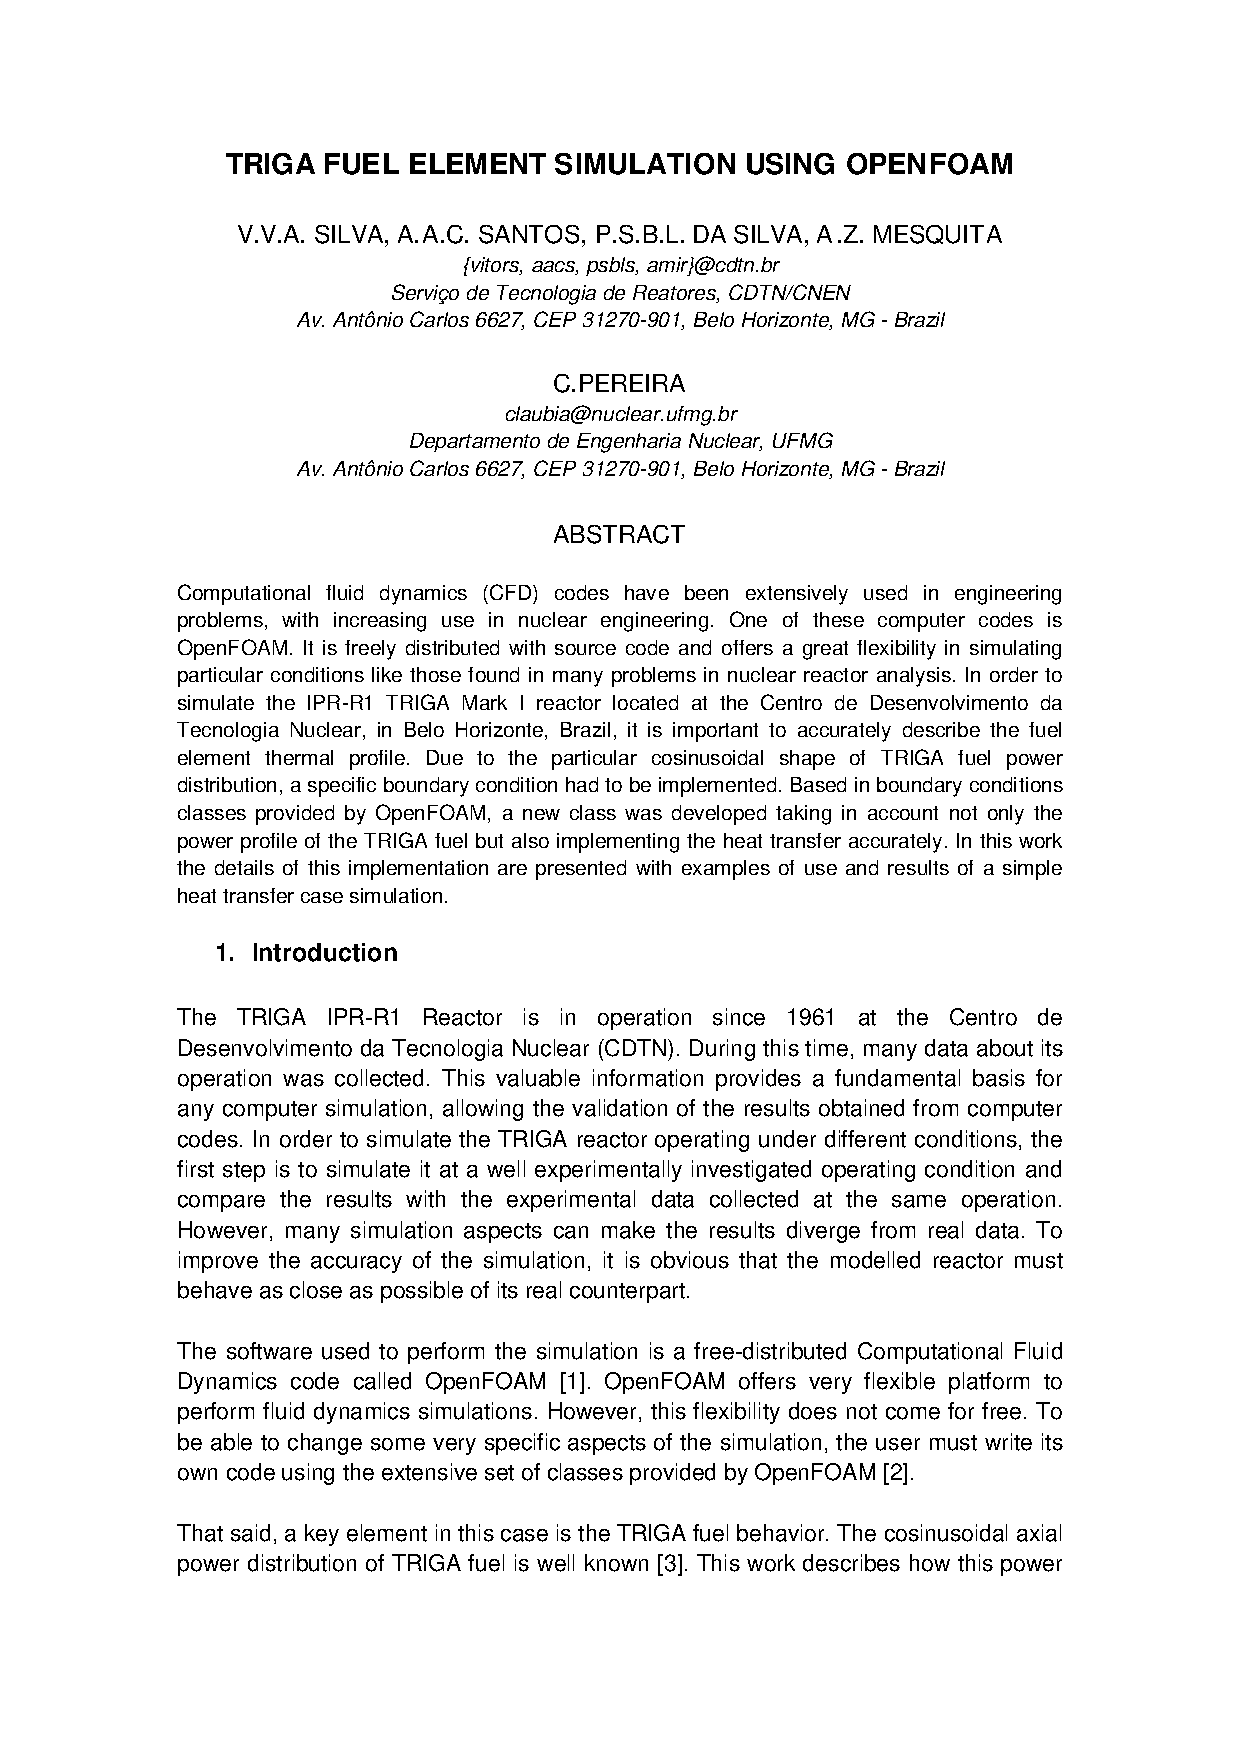
\includepdf[pages={-}]{anexos/RRFM2013.pdf}
%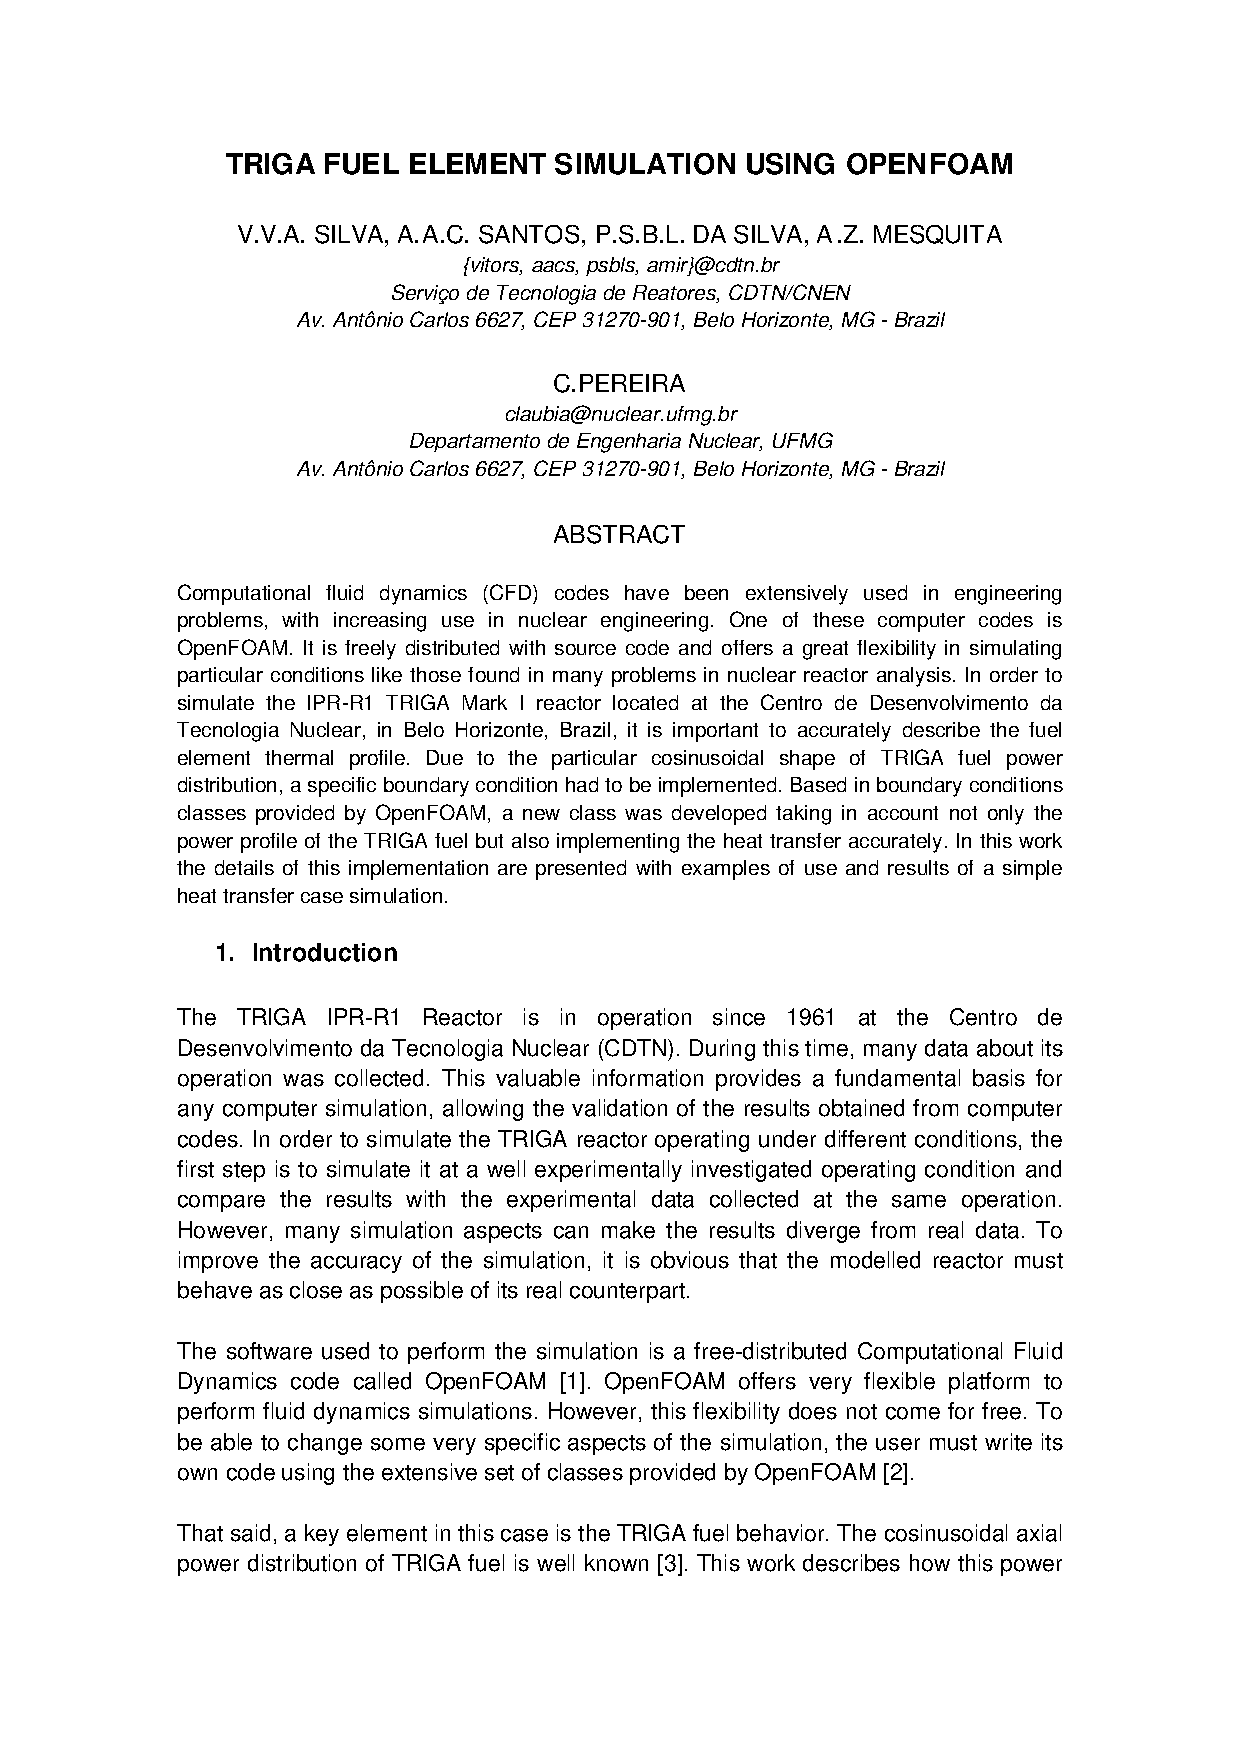
\includepdf[pages={1},pagecommand=\chapter{}]{anexos/RRFM2013.pdf}
%\includepdf[pages=2-,pagecommand={}]{anexos/RRFM2013.pdf}
\label{ane:RRFM2013}

%\chapter{Pedido do registro de Produto Tecnológico INPI}
\includepdf[pages={-}]{anexos/depositotrigafuel.pdf}
%\includepdf[pages={1},pagecommand=\chapter{}]{anexos/depositotrigafuel.pdf}
%\includepdf[pages=2-,pagecommand={}]{anexos/depositotrigafuel.pdf}
\label{ane:trigafuel}



\end{anexosenv}

%---------------------------------------------------------------------
% INDICE REMISSIVO
%---------------------------------------------------------------------

\printindex

\end{document}
